\documentclass[notes=show]{beamer}\usepackage[]{graphicx}\usepackage[]{color}
% maxwidth is the original width if it is less than linewidth
% otherwise use linewidth (to make sure the graphics do not exceed the margin)
\makeatletter
\def\maxwidth{ %
  \ifdim\Gin@nat@width>\linewidth
    \linewidth
  \else
    \Gin@nat@width
  \fi
}
\makeatother

\definecolor{fgcolor}{rgb}{0.345, 0.345, 0.345}
\newcommand{\hlnum}[1]{\textcolor[rgb]{0.686,0.059,0.569}{#1}}%
\newcommand{\hlstr}[1]{\textcolor[rgb]{0.192,0.494,0.8}{#1}}%
\newcommand{\hlcom}[1]{\textcolor[rgb]{0.678,0.584,0.686}{\textit{#1}}}%
\newcommand{\hlopt}[1]{\textcolor[rgb]{0,0,0}{#1}}%
\newcommand{\hlstd}[1]{\textcolor[rgb]{0.345,0.345,0.345}{#1}}%
\newcommand{\hlkwa}[1]{\textcolor[rgb]{0.161,0.373,0.58}{\textbf{#1}}}%
\newcommand{\hlkwb}[1]{\textcolor[rgb]{0.69,0.353,0.396}{#1}}%
\newcommand{\hlkwc}[1]{\textcolor[rgb]{0.333,0.667,0.333}{#1}}%
\newcommand{\hlkwd}[1]{\textcolor[rgb]{0.737,0.353,0.396}{\textbf{#1}}}%
\let\hlipl\hlkwb

\usepackage{framed}
\makeatletter
\newenvironment{kframe}{%
 \def\at@end@of@kframe{}%
 \ifinner\ifhmode%
  \def\at@end@of@kframe{\end{minipage}}%
  \begin{minipage}{\columnwidth}%
 \fi\fi%
 \def\FrameCommand##1{\hskip\@totalleftmargin \hskip-\fboxsep
 \colorbox{shadecolor}{##1}\hskip-\fboxsep
     % There is no \\@totalrightmargin, so:
     \hskip-\linewidth \hskip-\@totalleftmargin \hskip\columnwidth}%
 \MakeFramed {\advance\hsize-\width
   \@totalleftmargin\z@ \linewidth\hsize
   \@setminipage}}%
 {\par\unskip\endMakeFramed%
 \at@end@of@kframe}
\makeatother

\definecolor{shadecolor}{rgb}{.97, .97, .97}
\definecolor{messagecolor}{rgb}{0, 0, 0}
\definecolor{warningcolor}{rgb}{1, 0, 1}
\definecolor{errorcolor}{rgb}{1, 0, 0}
\newenvironment{knitrout}{}{} % an empty environment to be redefined in TeX

\usepackage{alltt}
\usepackage{amsmath}
\usepackage{graphicx}
\usepackage{mathpazo}
\usepackage{hyperref}
\usepackage{multimedia}
\usepackage{epstopdf}
\usepackage{tikz}
\usetikzlibrary{shapes,backgrounds}
\usepackage{multicol}

\setcounter{MaxMatrixCols}{10}
\usetheme{Madrid}


\newtheorem{conj}{Conjecture}[section]
\newtheorem{aim}{Aim}[section]
\newtheorem{remark}{Remark}[section]
\newtheorem{proposition}{Proposition}[section]
\newtheorem{interpretation}{Interpretation}[section]
\newtheorem{goal}{Goal}[section]
\newtheorem{exercise}{Exercise}[section]



\newcommand{\mbf}[1]{\mathbf{#1}}
\newcommand{\beq}{\begin{equation}}
\newcommand{\eeq}{\end{equation}}
\newcommand{\bea}{\begin{eqnarray}}
\newcommand{\eea}{\end{eqnarray}}
\newcommand{\ba}{\begin{array}}
\newcommand{\ea}{\end{array}}
\newcommand{\bi}{\begin{itemize}}
\newcommand{\ei}{\end{itemize}}
\newcommand{\ben}{\begin{enumerate}}
\newcommand{\een}{\end{enumerate}}
\newcommand{\nn}{\nonumber}
\newcommand{\fn}[1]{\footnote{#1}}
\renewcommand{\r}{\right}
\renewcommand{\l}{\left}
\long\def\symbolfootnote[#1]#2{\begingroup\def\thefootnote{\fnsymbol{footnote}}\footnote[#1]{#2}\endgroup}

%%%%%%%%%%%%%%%%%%%%%%%%%%%%%%%%%%%%%%%%%%%%%%%%%%%%%%%%%%%%%%%%%%%%%%%%%%%%%%%
% GSEM COLORS
%%%%%%%%%%%%%%%%%%%%%%%%%%%%%%%%%%%%%%%%%%%%%%%%%%%%%%%%%%%%%%%%%%%%%%%%%%%%%%%
\definecolor{darkGSEM}{RGB}{70,95,127}
\definecolor{darkGSEM2}{RGB}{40,80,150}
\definecolor{GSEM}{RGB}{96,121,153} % GSEM 10% lighter

%%% Global colors
\setbeamercolor*{palette primary}{use=structure,fg=white,bg=darkGSEM}
\setbeamercolor*{palette quaternary}{use=structure,fg=white,bg=darkGSEM!90}
\setbeamercolor{frametitle}{fg=white,bg=GSEM!80}

%%% TOC colors
\setbeamercolor{section in toc}{fg=darkGSEM}

%%% itemize colors
\setbeamertemplate{itemize items}[circle]
\setbeamercolor{itemize item}{fg=darkGSEM2}
\setbeamercolor{itemize subitem}{fg=darkGSEM2}
\setbeamercolor{itemize subsubitem}{fg=darkGSEM2}


%%% enumerate colors
\setbeamercolor{item projected}{fg=white,bg=GSEM}
\setbeamertemplate{enumerate item}{\insertenumlabel.}
\setbeamercolor{enumerate item}{fg=darkGSEM2}
\setbeamercolor{enumerate subitem}{fg=darkGSEM2}
\setbeamercolor{enumerate subsubitem}{fg=darkGSEM2}


\AtBeginSection[]
{
  \begin{frame}
    \frametitle{Outline}
    \tableofcontents[currentsection]
  \end{frame}
}

%%%%%%%%%%%%%%%%%%%%%%%%%%%%%%%%%%%%%%%%%%%%%%%%%%%%%%%%%%%%%%%%%%%%%%%%%%%%%%%%
\IfFileExists{upquote.sty}{\usepackage{upquote}}{}
\begin{document}
\title[S110015]{Probability 1}
\subtitle{Lecture 02 : Elements of Set Theory}
\author[Flores-Agreda, La Vecchia]{Dr. Daniel Flores-Agreda, \\[0.5em] \tiny{(based on the notes of Prof. Davide La Vecchia)}}
\date{Spring Semester 2021}

\begin{frame}
  \titlepage
\end{frame}


\begin{frame}
\frametitle{Objective}
  Kickstart the mathematical characterisation of probability by:\\[1.5em]
  \begin{itemize}
  \item Introducing: \textbf{Random Experiments, Events, and Sample Spaces} and characterising them as \textbf{Sets}.\\[1em]
  \item Providing \textbf{elements of Set Theory} helpful in the study of probability.\\[1em]
  \item Giving an informal definition Probability as \textbf{Frequency}.
  \end{itemize}
\end{frame}

\begin{frame}
\frametitle{Outline}
\tableofcontents
\end{frame}




%%%%%%%%%%%%%%%%%%%%%%%%%%%%%%
\section{Random Experiments, Events and Sample Spaces}
%%%%%%%%%%%%%%%%%%%%%%%%%%%%%%

\begin{frame}{\secname}
\framesubtitle{Definitions}
  \begin{definition}
  A \textcolor{blue}{random experiment} is a process that can \textbf{result in two or more different outcomes} with \textbf{uncertainty} as to which will be observed.
  \end{definition}
  \pause
  \begin{example}
    \begin{center}
    Drawing a card in a BlackJack game.
    \end{center}
  \end{example}
\end{frame}

\begin{frame}{\secname}
  \framesubtitle{Definitions}
  \begin{definition}
  An \textcolor{blue}{event} is an \textbf{uncertain outcome} of a random experiment.
  \end{definition}
  \pause
  \begin{example}
    \begin{center}
    The card drawn is a \textcolor{red}{King of Hearts}
    \end{center}
  \end{example}
  \pause
  An event can be:
  \begin{itemize}
  \item \textbf{Elementary}: includes \textbf{only one particular outcome}.
  \item \textbf{Composite}: includes \textbf{more than one elementary outcome}.
  \end{itemize}
\end{frame}

\begin{frame}{\secname}
\framesubtitle{Definitions}
  \begin{definition}
  The \textcolor{blue}{Sample Space}($S$) is the complete \textbf{listing of the elementary events} that can occur in a random experiment.
  \end{definition}
\end{frame}

\begin{frame}{\secname}
\framesubtitle{Examples}
  \begin{example}[Drawing a single card from a deck]
  \begin{figure}[h!]
  \centering
  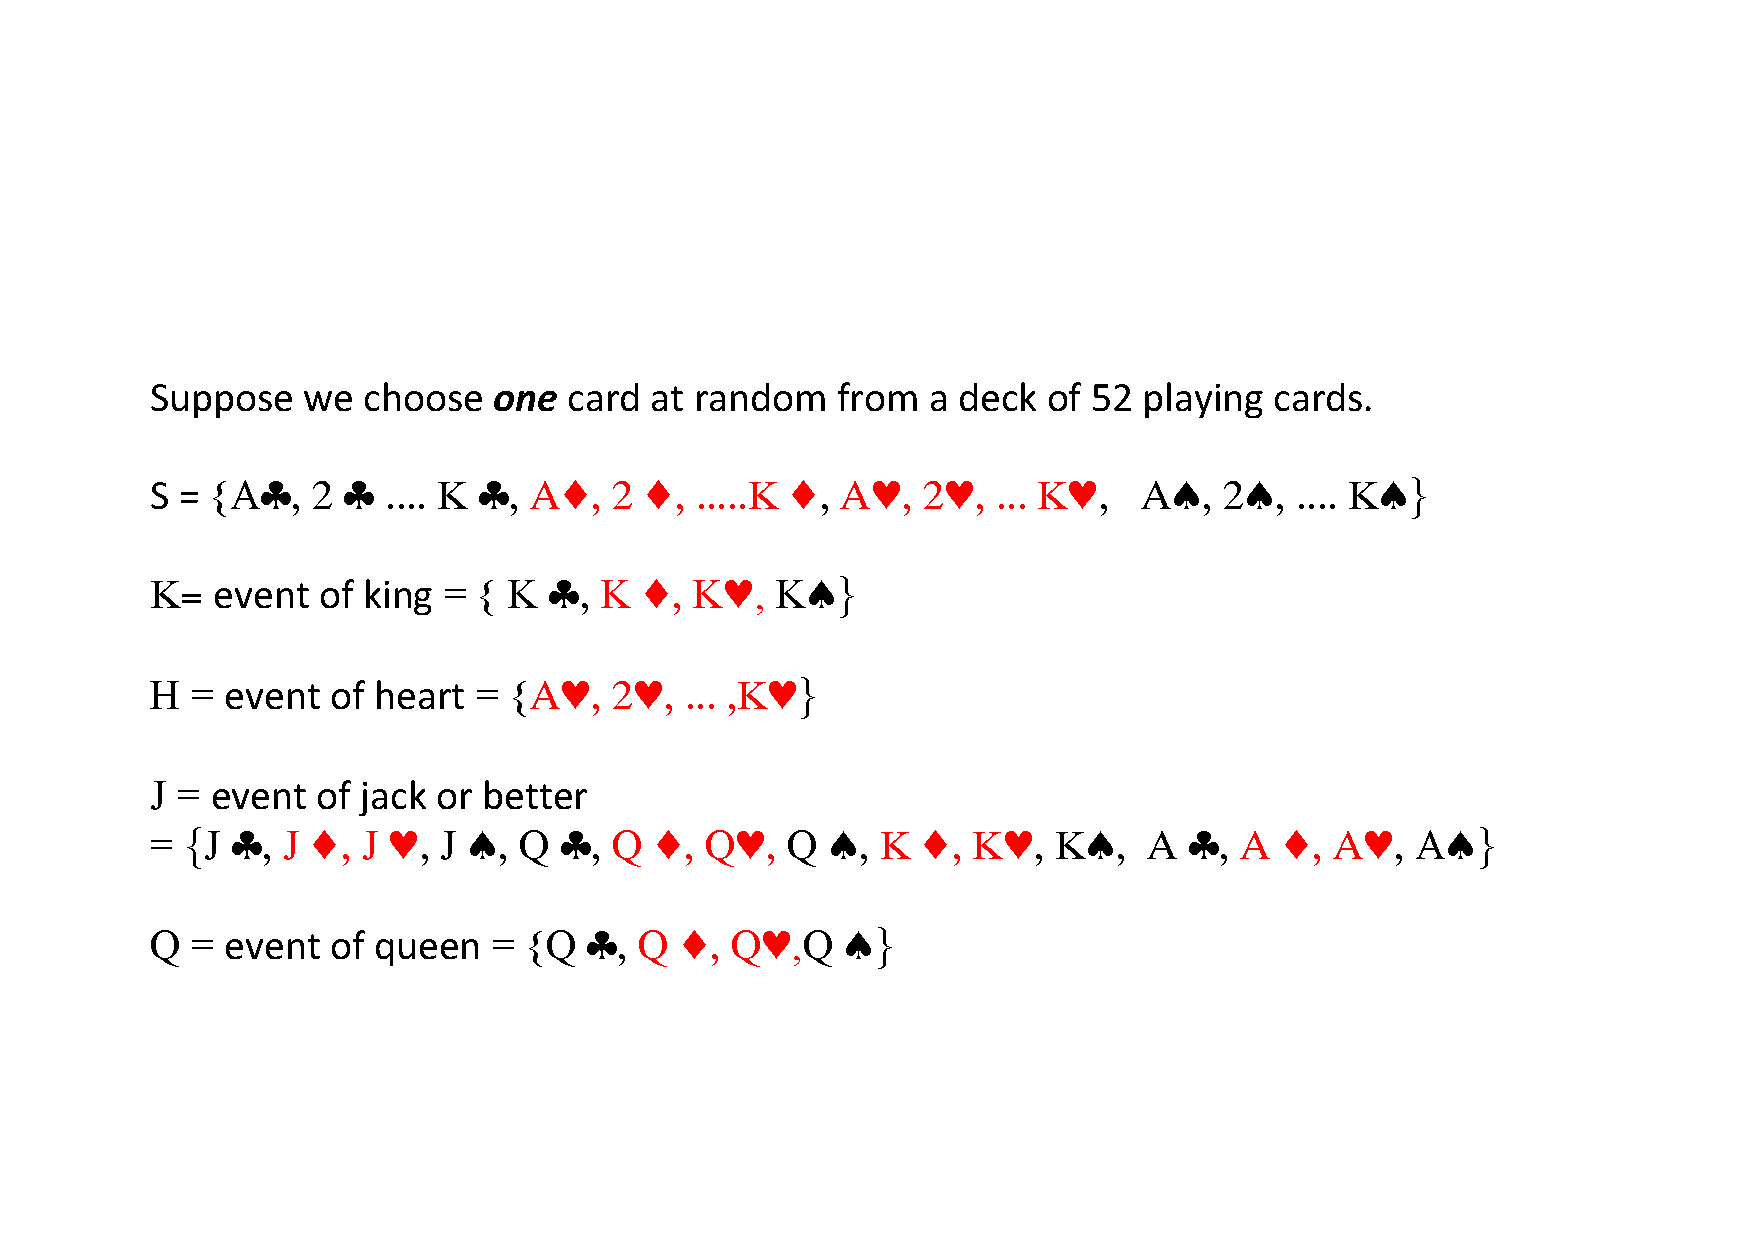
\includegraphics[width=0.9\textwidth,height=0.55\textheight]{img/Example1_GE.pdf}
  \end{figure}
  \end{example}
\end{frame}

\begin{frame}{\secname}
\framesubtitle{Examples}
  \begin{example}[Tossing two coins]
  \begin{itemize}
  \item Flipping two coins, could be seen as an \textbf{Experiment}

  \pause

  \item If we flip two coins and name:
  \begin{itemize}
  \item $H$ for Head and
  \item $T$ for Tail,
  \end{itemize}
  each of these pairs, e.g. $(H,T)$ constitutes an \textbf{Outcome}.

  \pause

  \item Hence, the \textbf{Sample Space} contains the following four points:
  $$ S = \{ (HH),(HT),(TH),(TT)  \}.$$
  \end{itemize}
  \end{example}
\end{frame}

\begin{frame}{\secname}
\framesubtitle{Examples}
  \begin{example}[Measuring time on screen]
  \begin{itemize}
  \item Taking a measure of time spent on your Phone, can be considered an \textbf{experiment}.

  \item \textbf{Outcomes} are positive measures


  \item The \textbf{Sample Space} consists of all non-negative real numbers:
  $$
  S = \{x: 0 \leq x < \infty \} \equiv \mathbb{R}^+
  $$
  \end{itemize}
  \end{example}
\end{frame}

%%%%%%%%%%%%%%%%%%%%%%%%%%
\section{Some Definitions from Set Theory}
%%%%%%%%%%%%%%%%%%%%%%%%%%

\begin{frame}{\secname}

Since events are seen as sets, we rely on set theory to study them further.
\pause
\begin{definition}
\begin{itemize}
\item If every element of a set $A$ is also an element of a set $B$, then \textbf{$A$ is a subset of $B$}: $$ A \subset B,$$ read as ``$A$ is contained in $B$''
\item Two sets $A$ and $B$ are \textbf{equal} if $$A \subset B \text{ \ and \ } B \subset A;$$
\item If a set $A$ contains \textbf{no elements}, it's a \textit{null set, or empty set}, and denoted by $\varnothing$.
\end{itemize}
\end{definition}
\end{frame}


%\begin{frame}
%\frametitle{Some definitions from set theory}
%
%
%\end{frame}

%%%%%%%%%%%%%%%%%%%%%%%%%%%%%%%%%%
\section{The Venn Diagram}
%%%%%%%%%%%%%%%%%%%%%%%%%%%%%%%%%%

\begin{frame}{\secname}
\begin{figure}[h!]
\centering
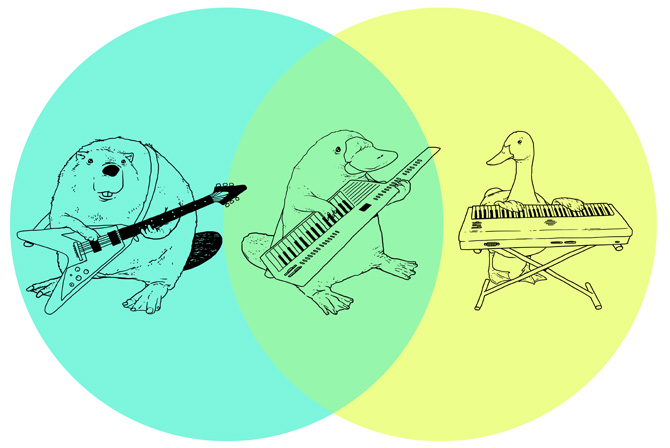
\includegraphics[scale=0.4]{../../book/img/fun/R9mJR.jpeg}
\end{figure}
\end{frame}


\begin{frame}{\secname}
A Venn diagram is an enclosed figure representing a set.

It helps us show basic features of a given set.
\begin{figure}[h!]
\centering
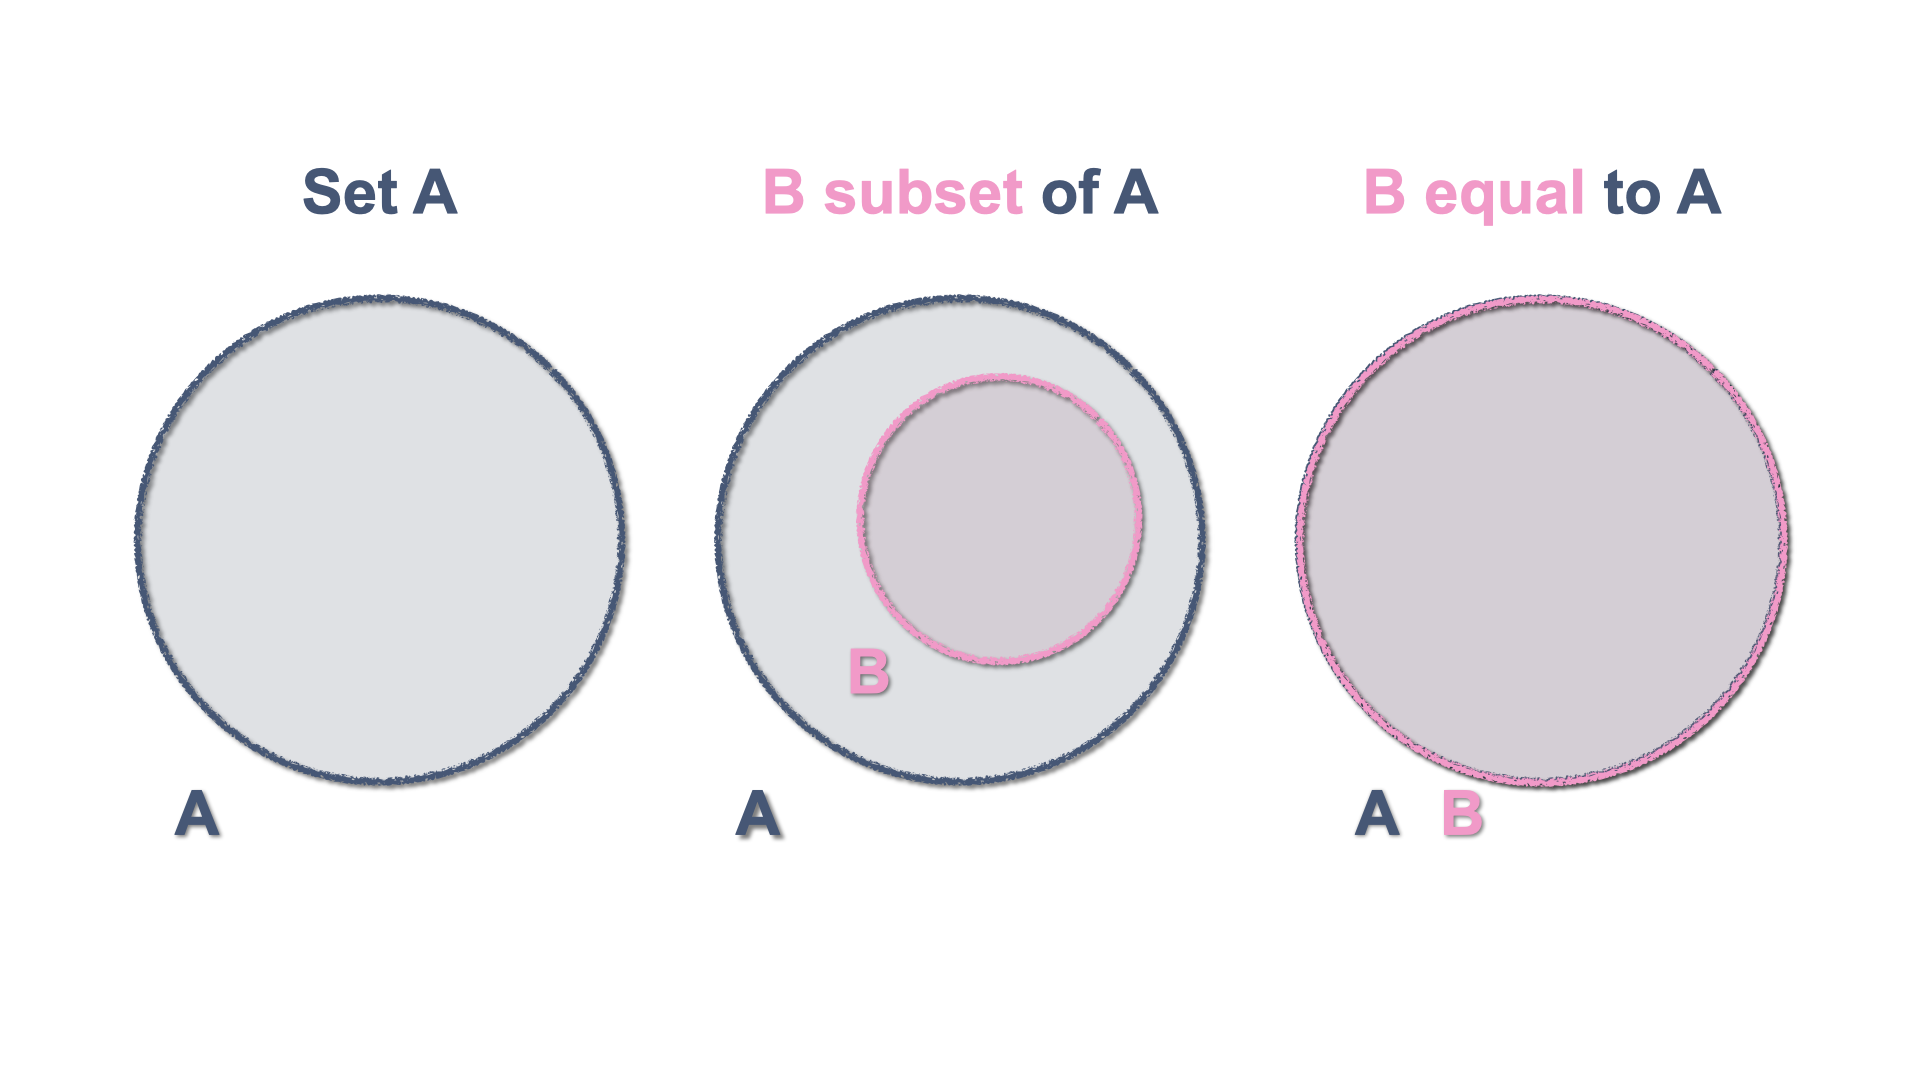
\includegraphics[width=0.8\textwidth,height=0.6\textheight]{img/charts/charts.001.png}
\end{figure}

\end{frame}

\begin{frame}
\frametitle{The Venn Diagram}

We will use Venn Diagrams to represent \textbf{Events in the Sample Space}

\begin{figure}[h!]
\centering
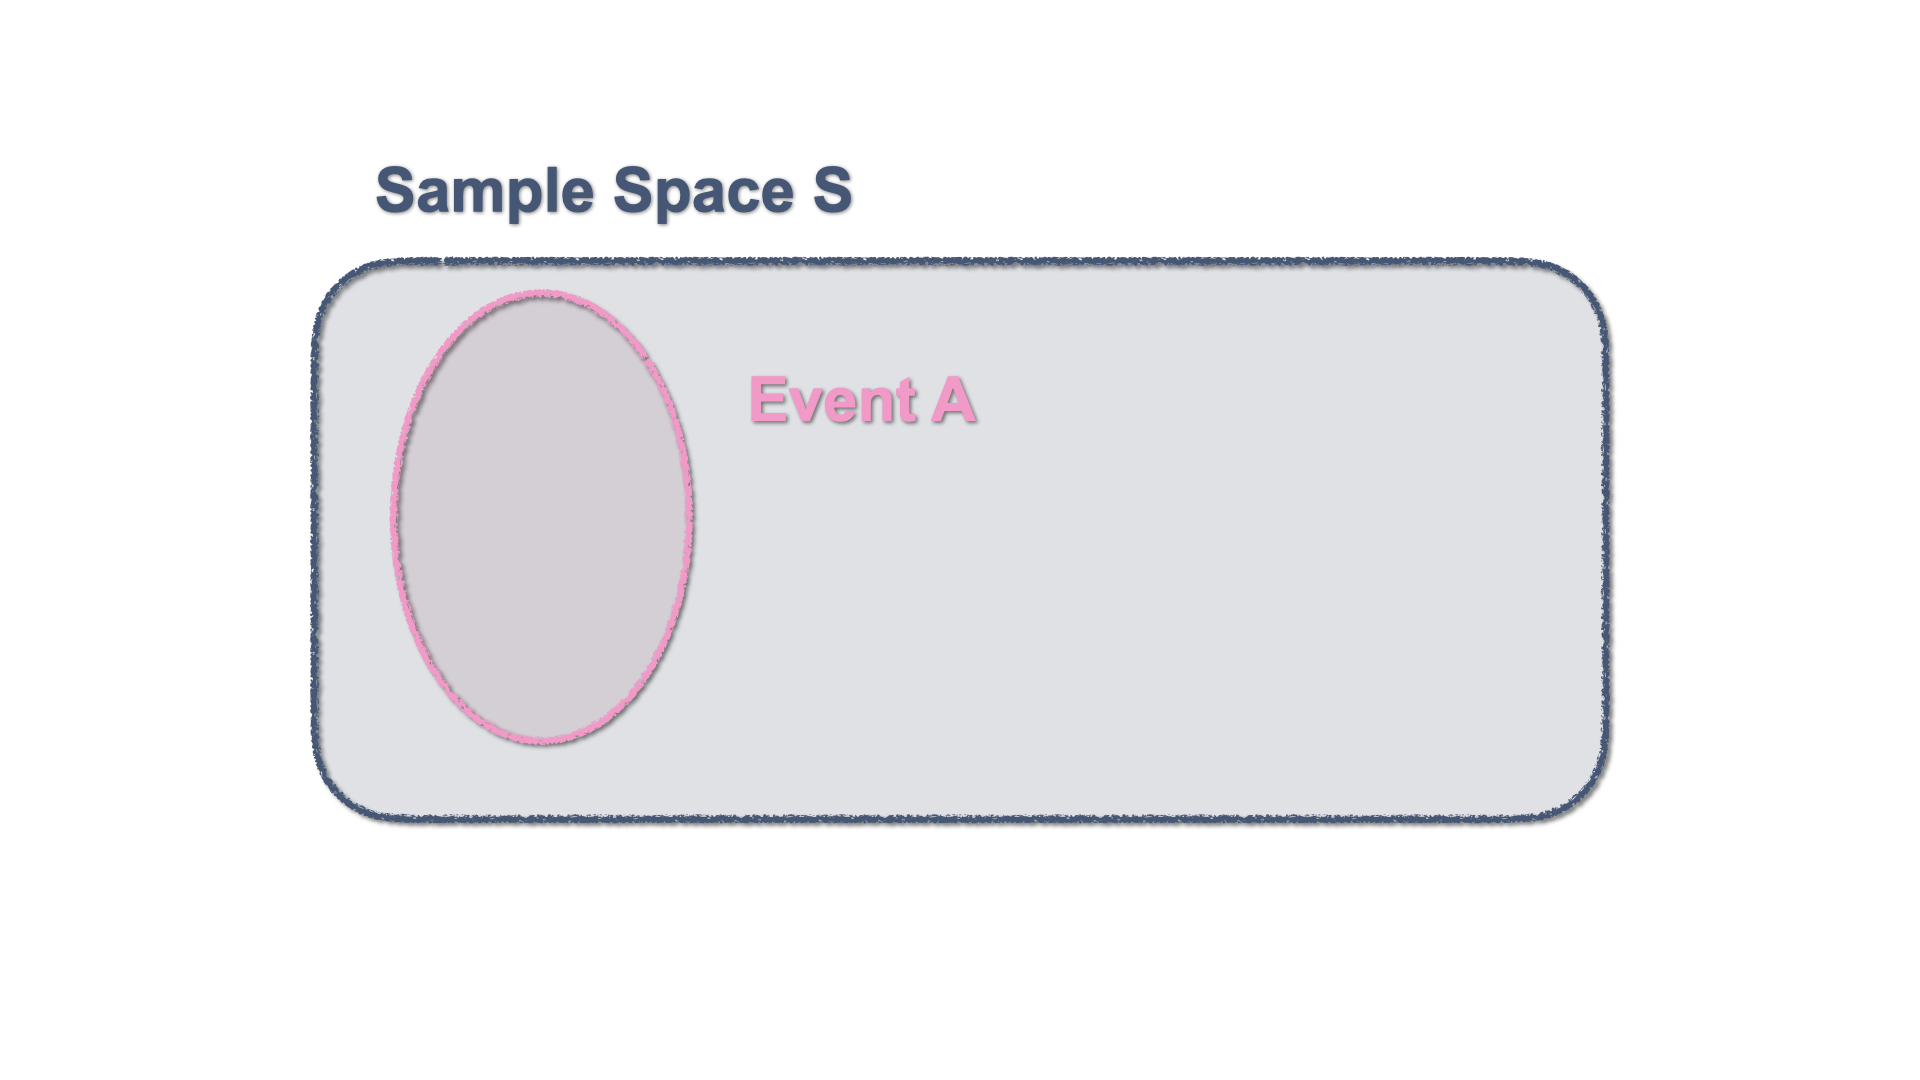
\includegraphics[width=0.8\textwidth,height=0.6\textheight]{img/charts/charts.002.png}
\end{figure}
\end{frame}



\begin{frame}
\frametitle{The Venn Diagram}


Two events are \textbf{mutually exclusive} is they cannot occur jointly.

\begin{figure}[h!]
\centering
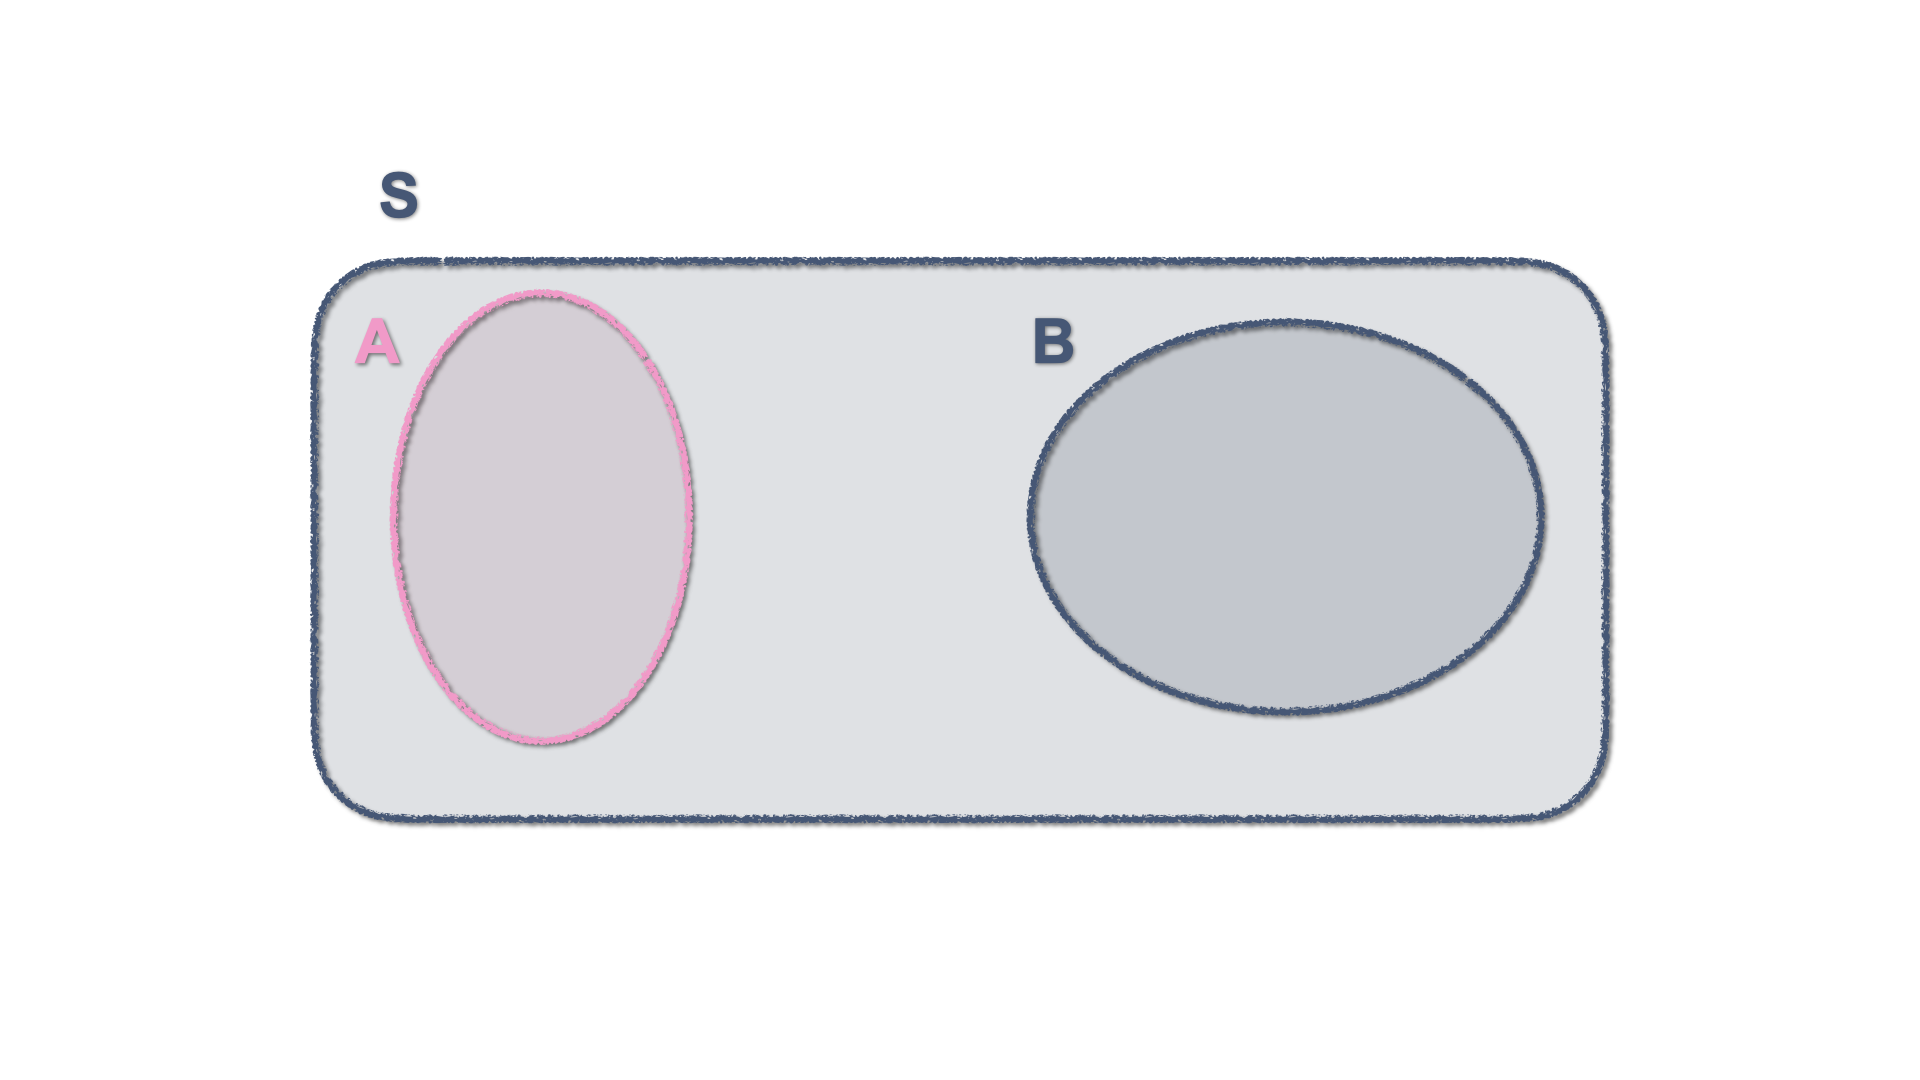
\includegraphics[width=1\textwidth,height=0.7\textheight]{img/charts/charts.003.png}
\end{figure}
\end{frame}

\begin{frame}
\frametitle{Elements of set theory (Venn diagram)}

Two events are \textbf{not mutually exclusive} if they share some elements.


\begin{figure}[h!]
\centering
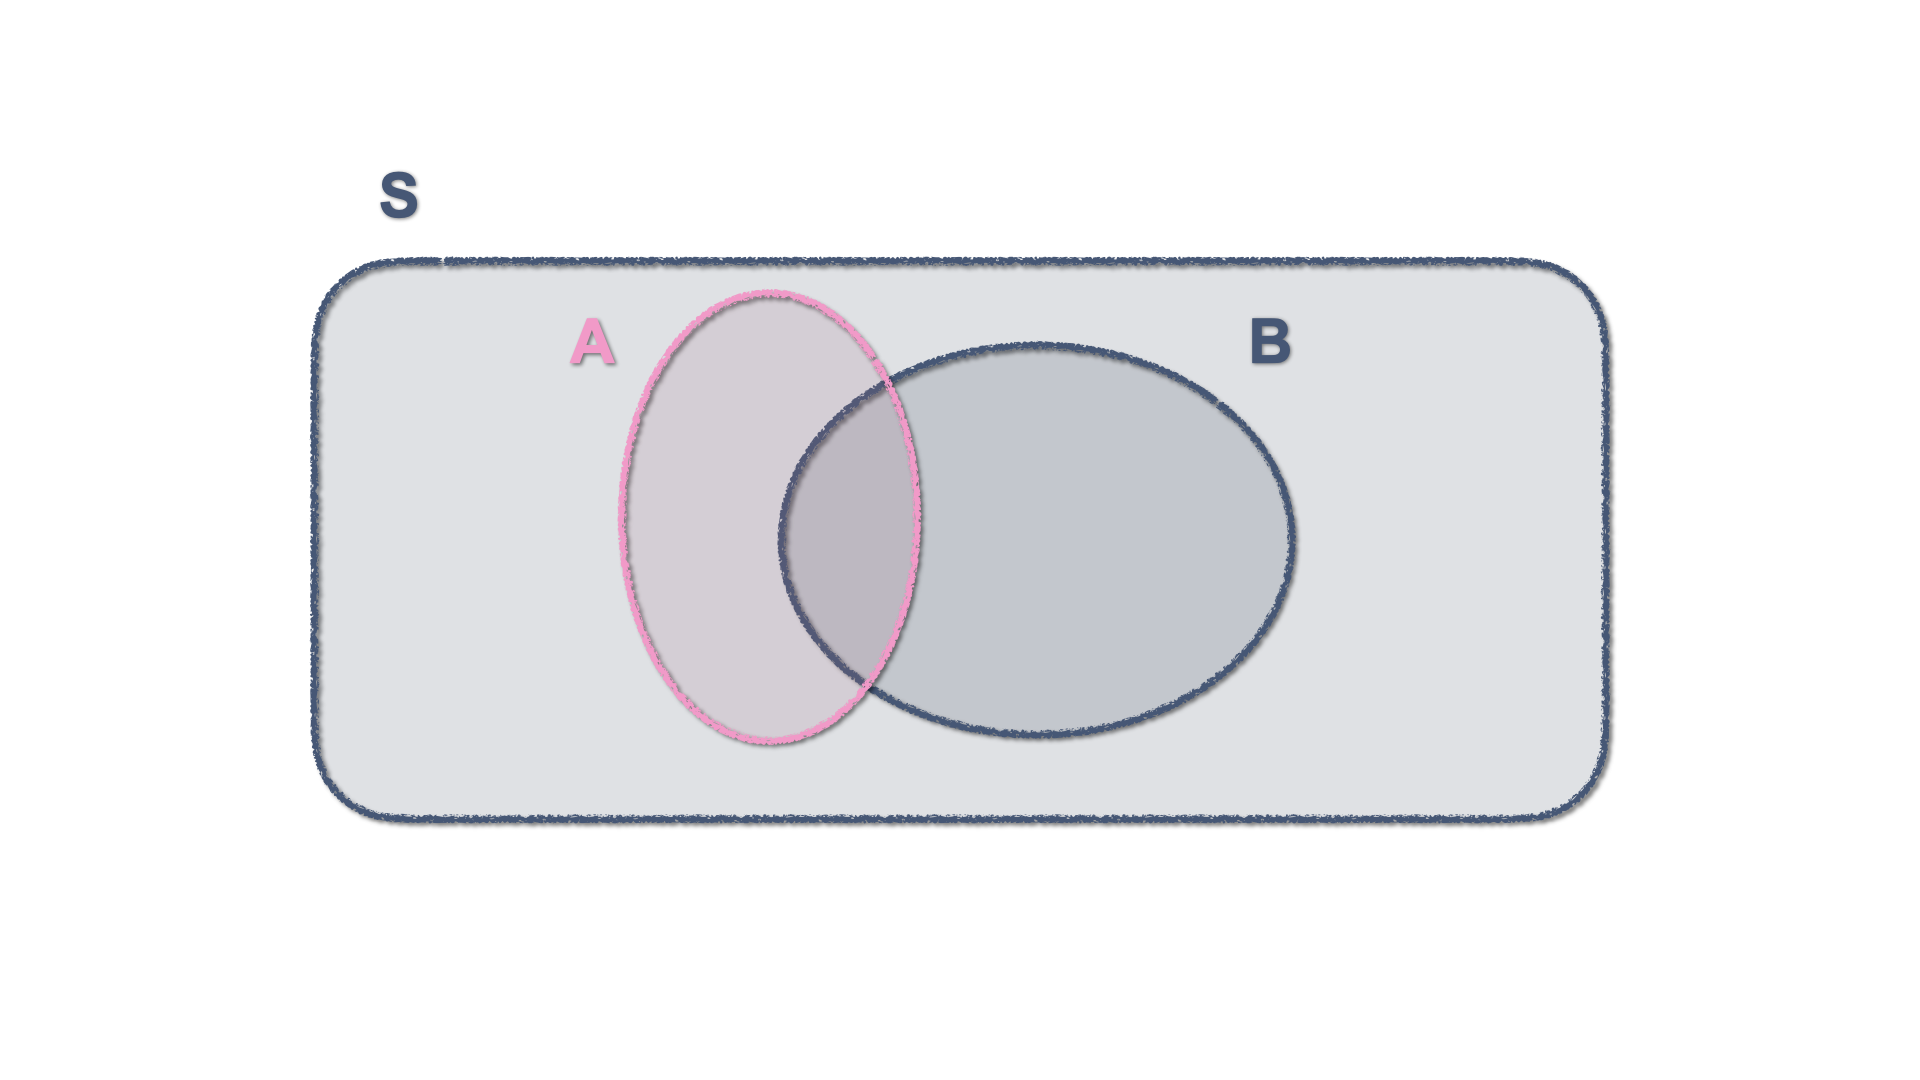
\includegraphics[width=1\textwidth,height=0.7\textheight]{img/charts/charts.004.png}
\end{figure}
\end{frame}


\begin{frame}
\frametitle{The Venn Diagram}

The \textbf{union of the events} $A$ and $B$ is the event which \textbf{occurs when either $A$ or $B$ occurs}: $A \cup B$
\begin{figure}[h!]
\centering
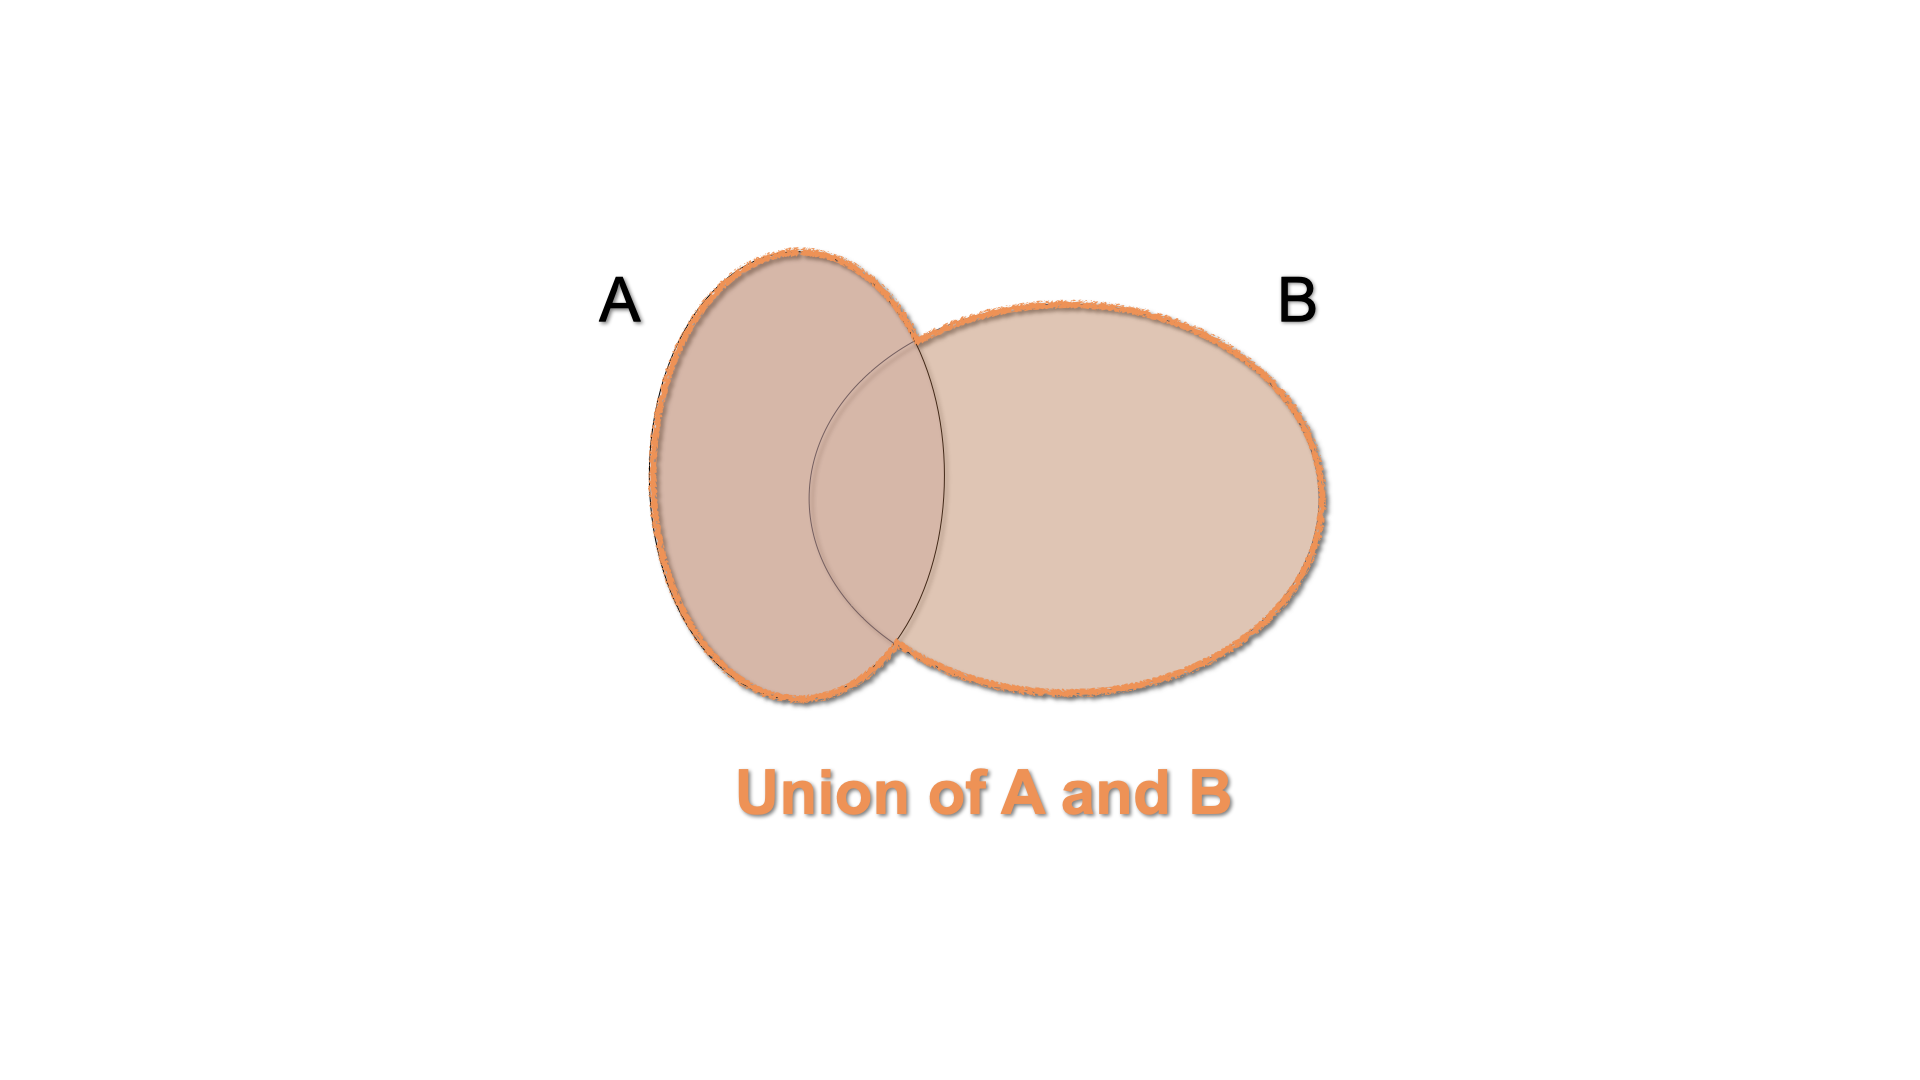
\includegraphics[width=1\textwidth,height=0.7\textheight]{img/charts/charts.005.png}
\end{figure}
% \vspace{1cm}
% \hspace{2cm}
% \def\firstcircle{(0,0) circle (1.5cm)}
% \def\secondcircle{(45:2cm) circle (1.5cm)}
% \begin{tikzpicture}
%     \begin{scope}[shift={(6cm,5cm)}, fill opacity=0.65]
%         \fill[blue!20] \firstcircle;
%         \fill[blue!20] \secondcircle;
%         \draw \firstcircle node[below] {$A$};
%         \draw \secondcircle node [above] {$B$};
% %        \draw node [above] {$A \cup B$}
%     \end{scope}
% \end{tikzpicture}

\end{frame}


\begin{frame}
\frametitle{The Venn Diagram}

The intersection of the events $A$ and $B$ is the event which occurs when both $A$ and $B$ occur: $A \cap B$\\

\begin{figure}[h!]
\centering
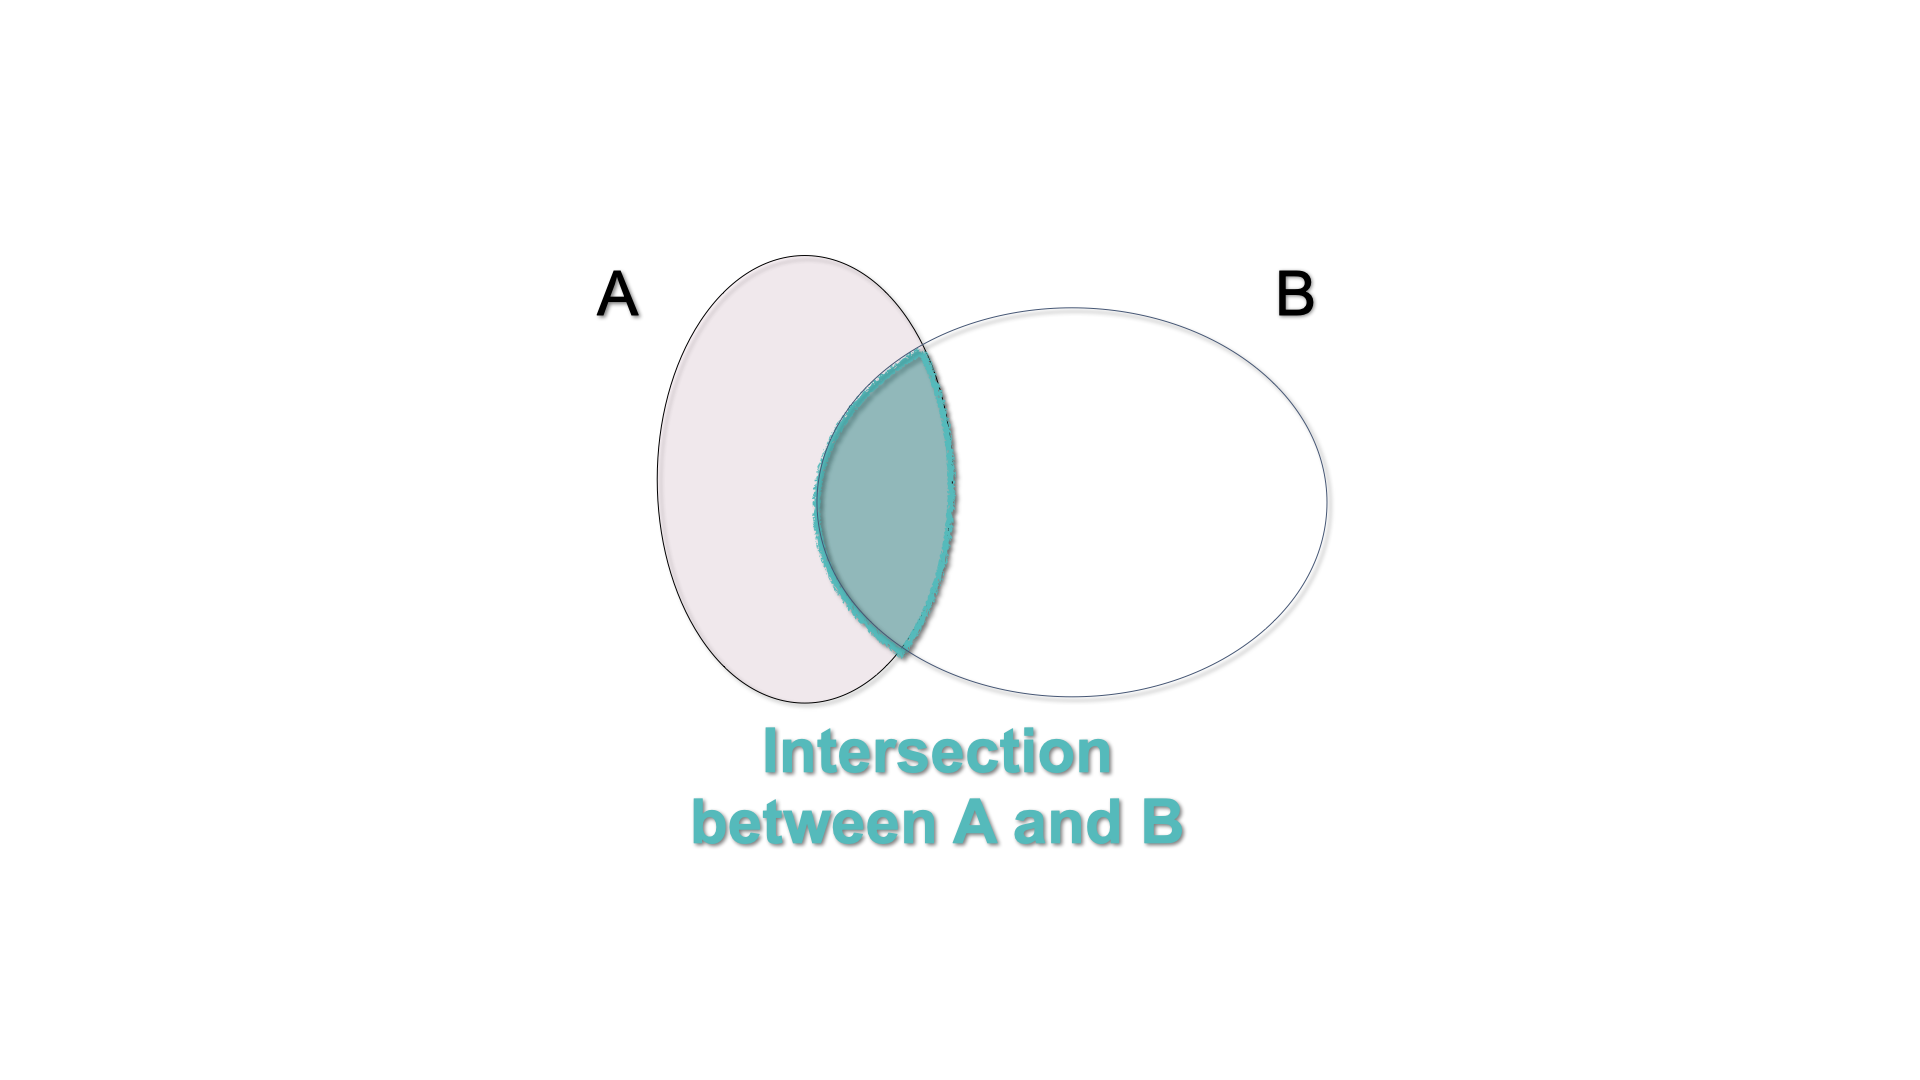
\includegraphics[width=1\textwidth,height=0.7\textheight]{img/charts/charts.006.png}
\end{figure}

% \vspace{1cm}
% \hspace{2cm}
% \def\firstcircle{(0,0) circle (1.5cm)}
% \def\secondcircle{(45:2cm) circle (1.5cm)}
% \begin{tikzpicture}
%     \begin{scope}[shift={(6cm,5cm)}, fill opacity=0.65]
%     \draw \firstcircle node[below] {$A$};
%     \draw \secondcircle node [above] {$B$};
%
%       \clip \firstcircle;
%       \fill[blue!20] \secondcircle;
%     \end{scope}
% \end{tikzpicture}


\end{frame}


%\begin{frame}
%\frametitle{Elements of set theory (Venn diagram)}
%
%The intersection of the events $A$ and $B$ is the event which occurs when both $A$ and $B$ occur: $A \cap B$
%
%\begin{figure}[h!]
%\centering
%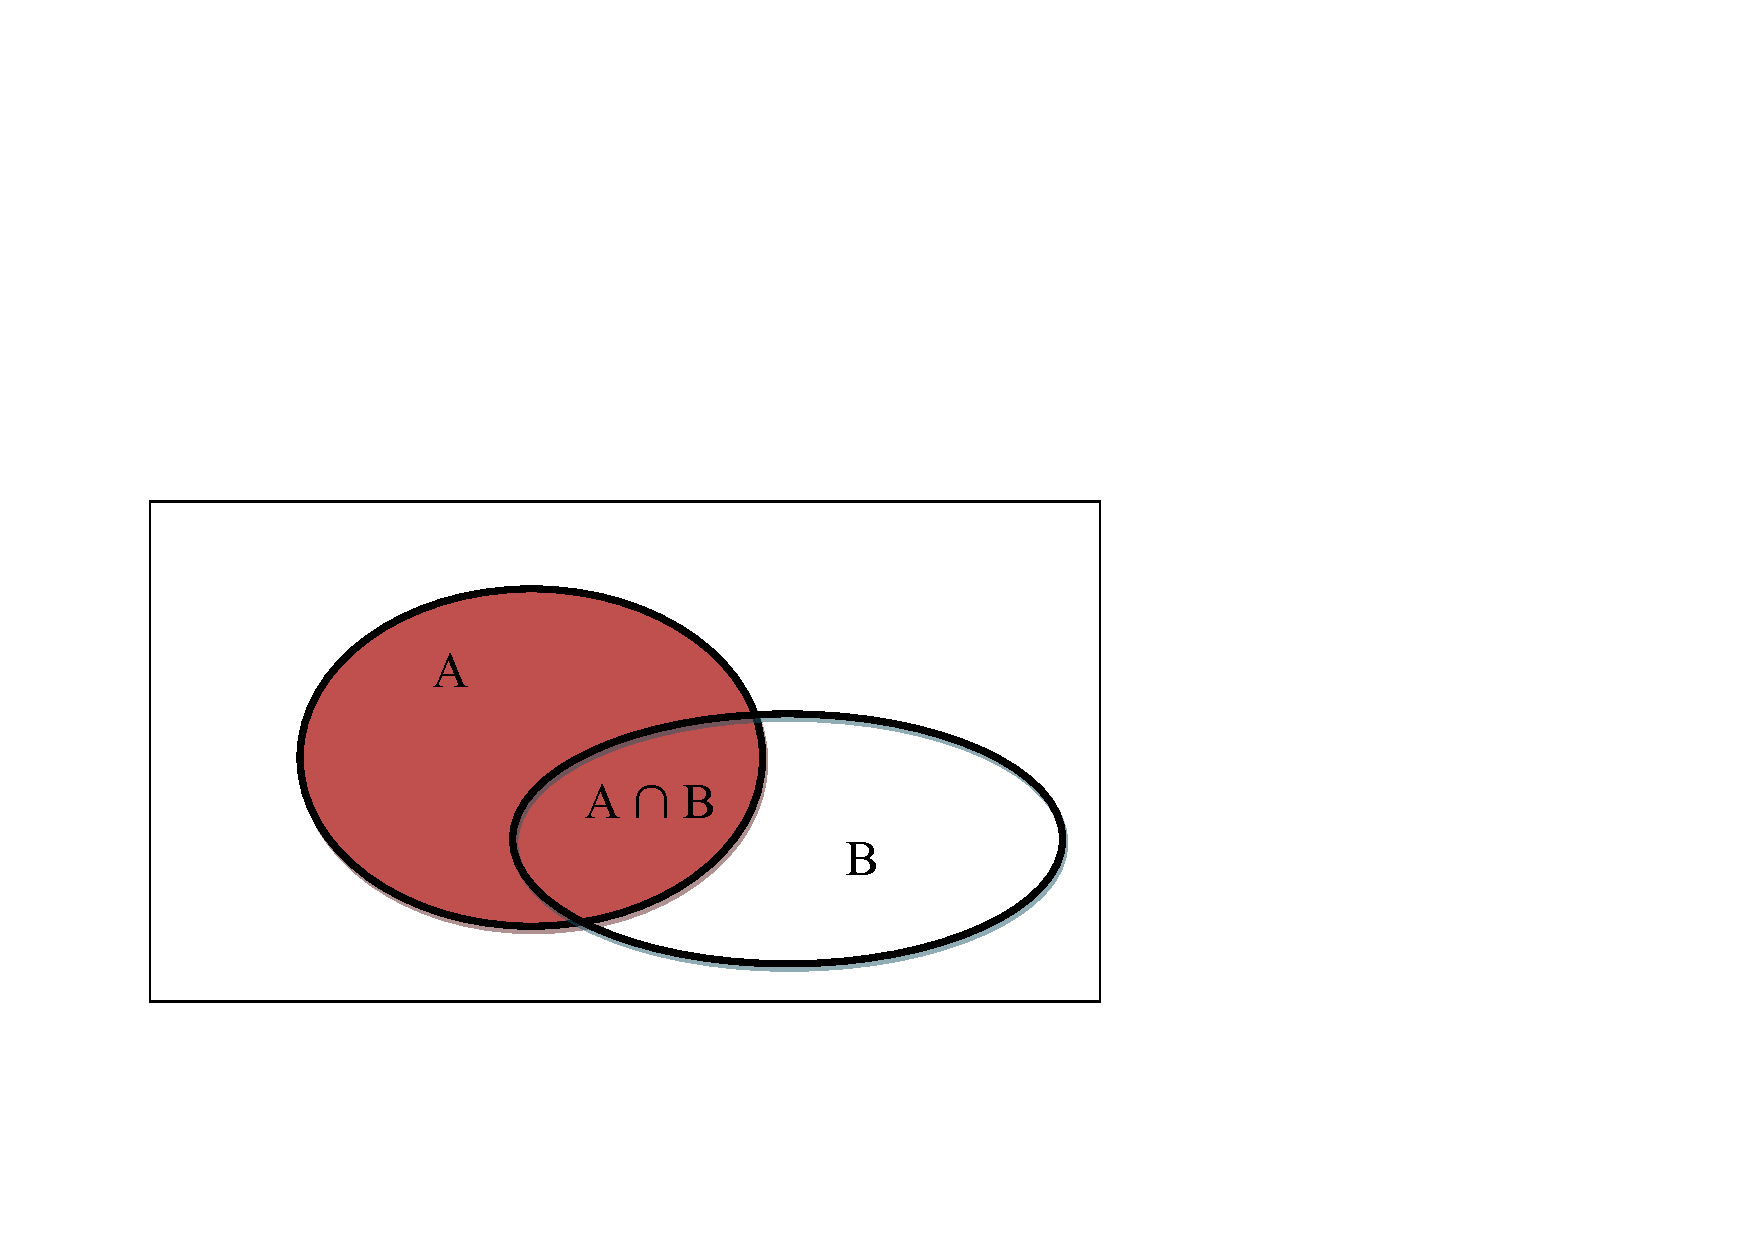
\includegraphics[width=1\textwidth,height=0.7\textheight]{Venn5.pdf}
%\end{figure}
%\end{frame}

\begin{frame}{\secname}
The complement of an event $A$ is the event which occurs when $A$ does not occur: $A^{c}$ (or $\overline{A}$)
\pause
\begin{figure}[h!]
\centering
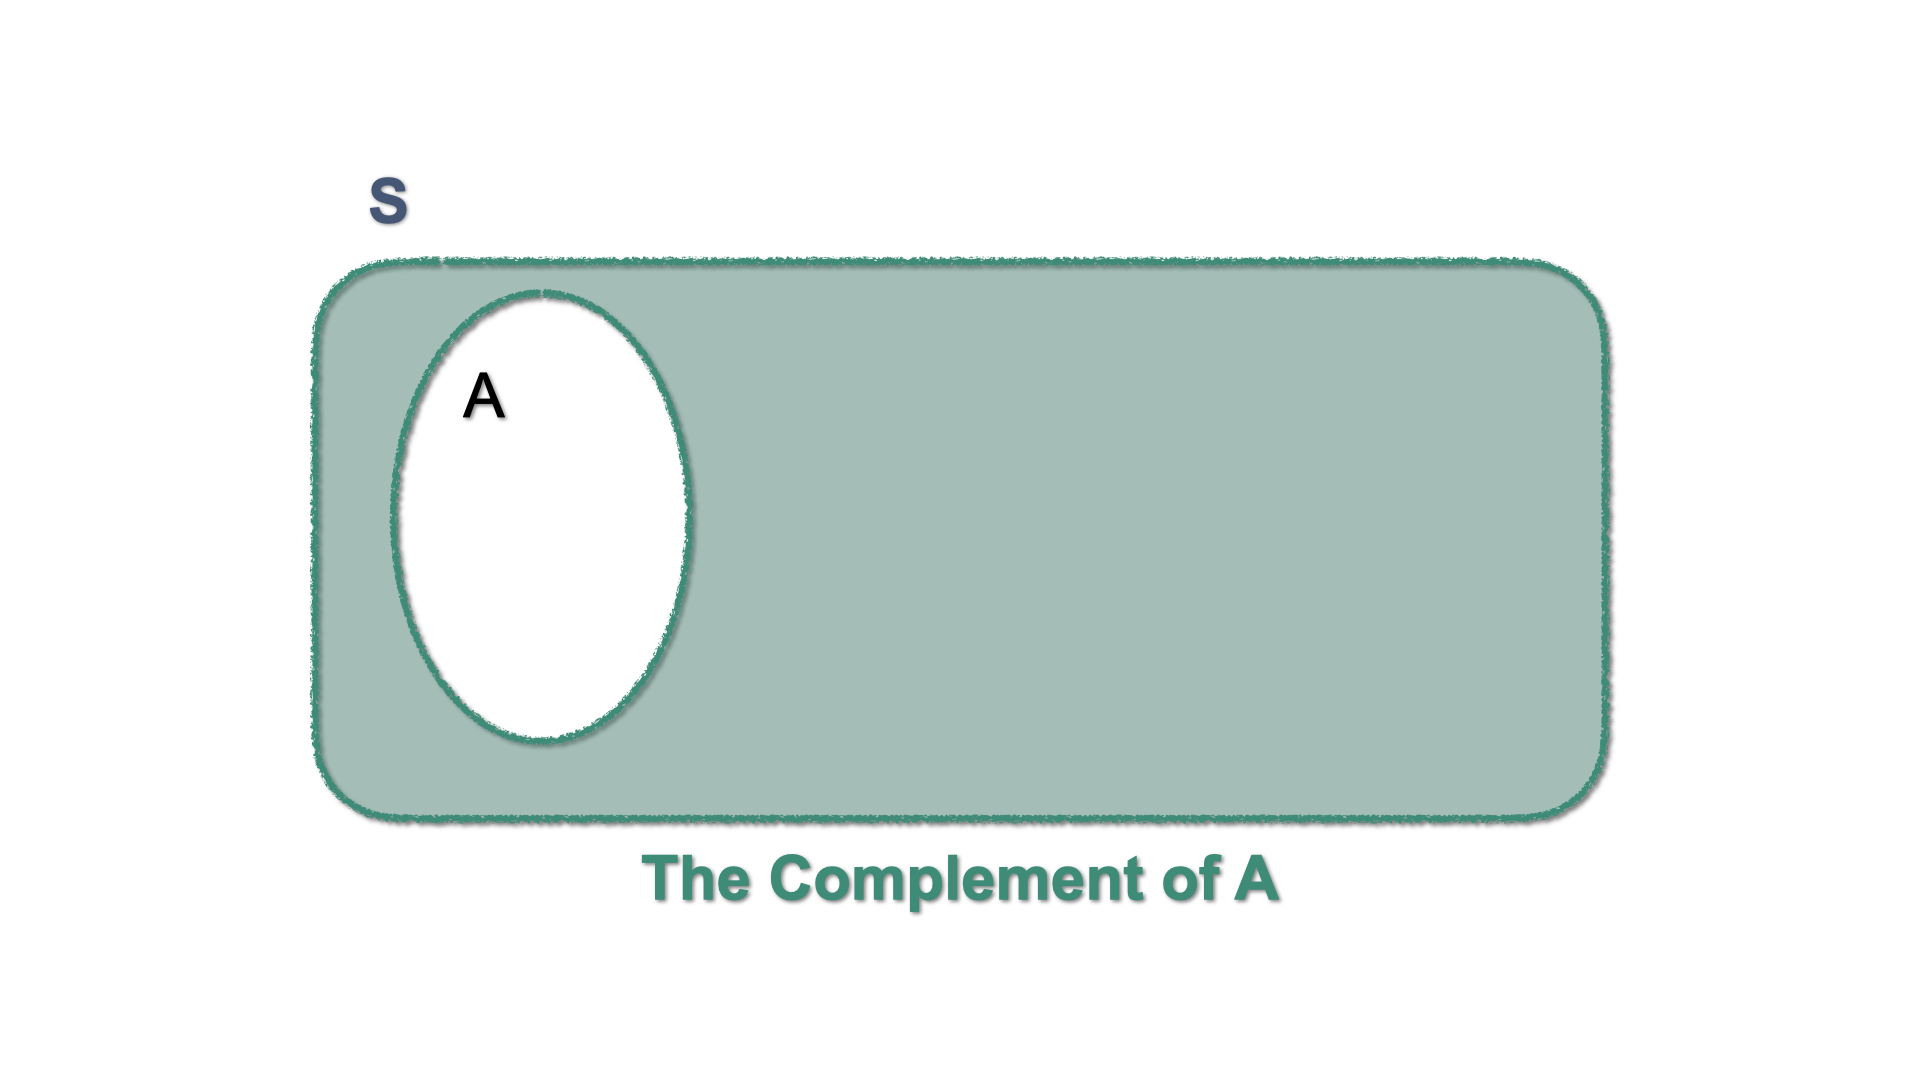
\includegraphics[scale=0.1]{img/charts/charts.007.png}
\end{figure}
\pause
\begin{center}
$A \cup A^c = S$ and $A^c = S \setminus A = S-A$.
\end{center}
\end{frame}

\begin{frame}{\secname}
Let $A$, $B$, and $C$ be sets. The following laws hold:
\begin{itemize}
\item \textbf{Commutative laws}:
\begin{eqnarray*}
A \cup B = B \cup A \\
A \cap B = B \cap A
\end{eqnarray*}
\item \textbf{Associative laws}:
\begin{eqnarray*}
A \cup (B \cup C) = (A \cup B) \cup C \\
A \cap (B \cap C) = (A \cap B) \cap C
\end{eqnarray*}
\end{itemize}
\end{frame}

\begin{frame}{\secname}
  \textbf{Distributive laws}:
  \begin{center}
  \textit{The intersection is distributive with respect to the union}
  \end{center}
  $$A \cap (B \cup C) = (A \cap B) \cup (A\cap C)$$
  \begin{figure}[h!]
  \centering
  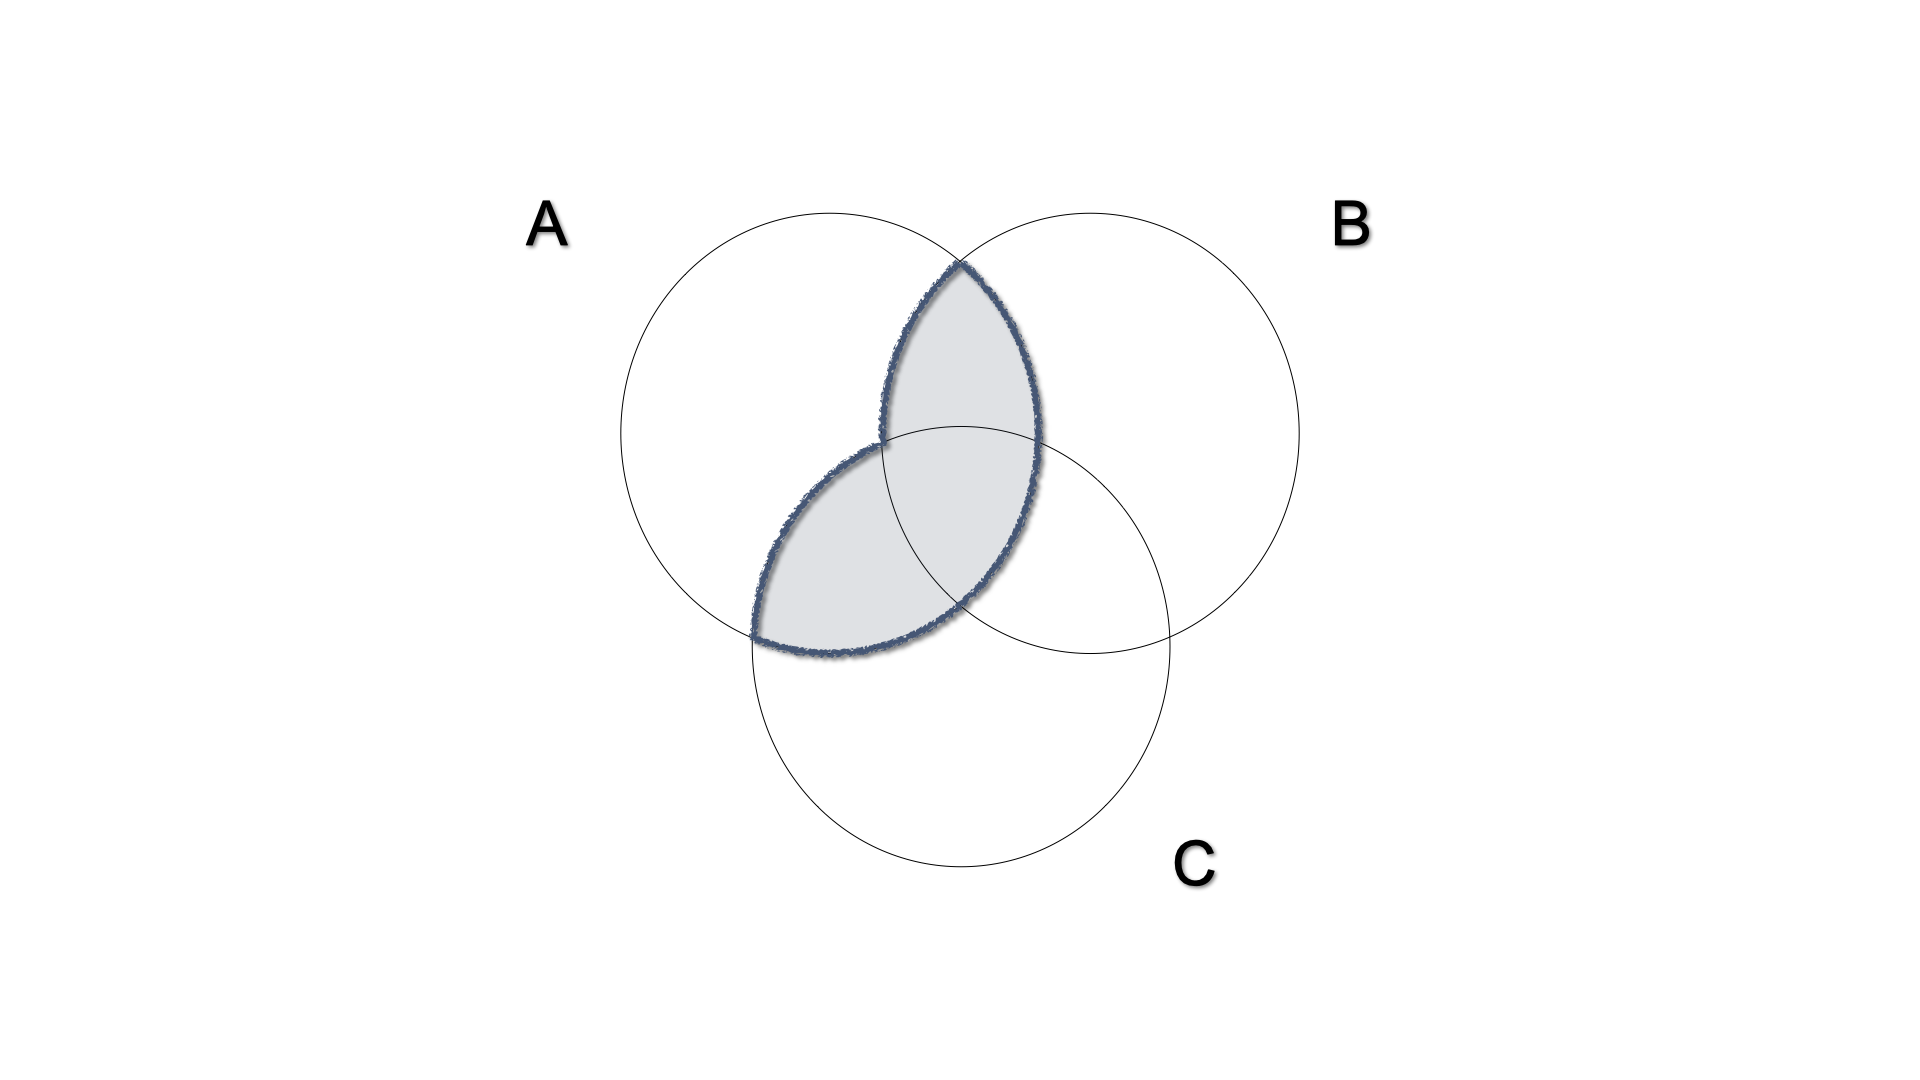
\includegraphics[scale=0.15]{img/charts/charts.008.png}
  \end{figure}
\end{frame}

\begin{frame}{\secname}
  \textbf{Distributive laws}:
  \begin{center}
  \textit{The union is distributive with respect to the intersection}
  \end{center}
  $$A \cup (B \cap C) = (A\cup B) \cap (A \cup C)$$
  \begin{figure}[h!]
  \centering
  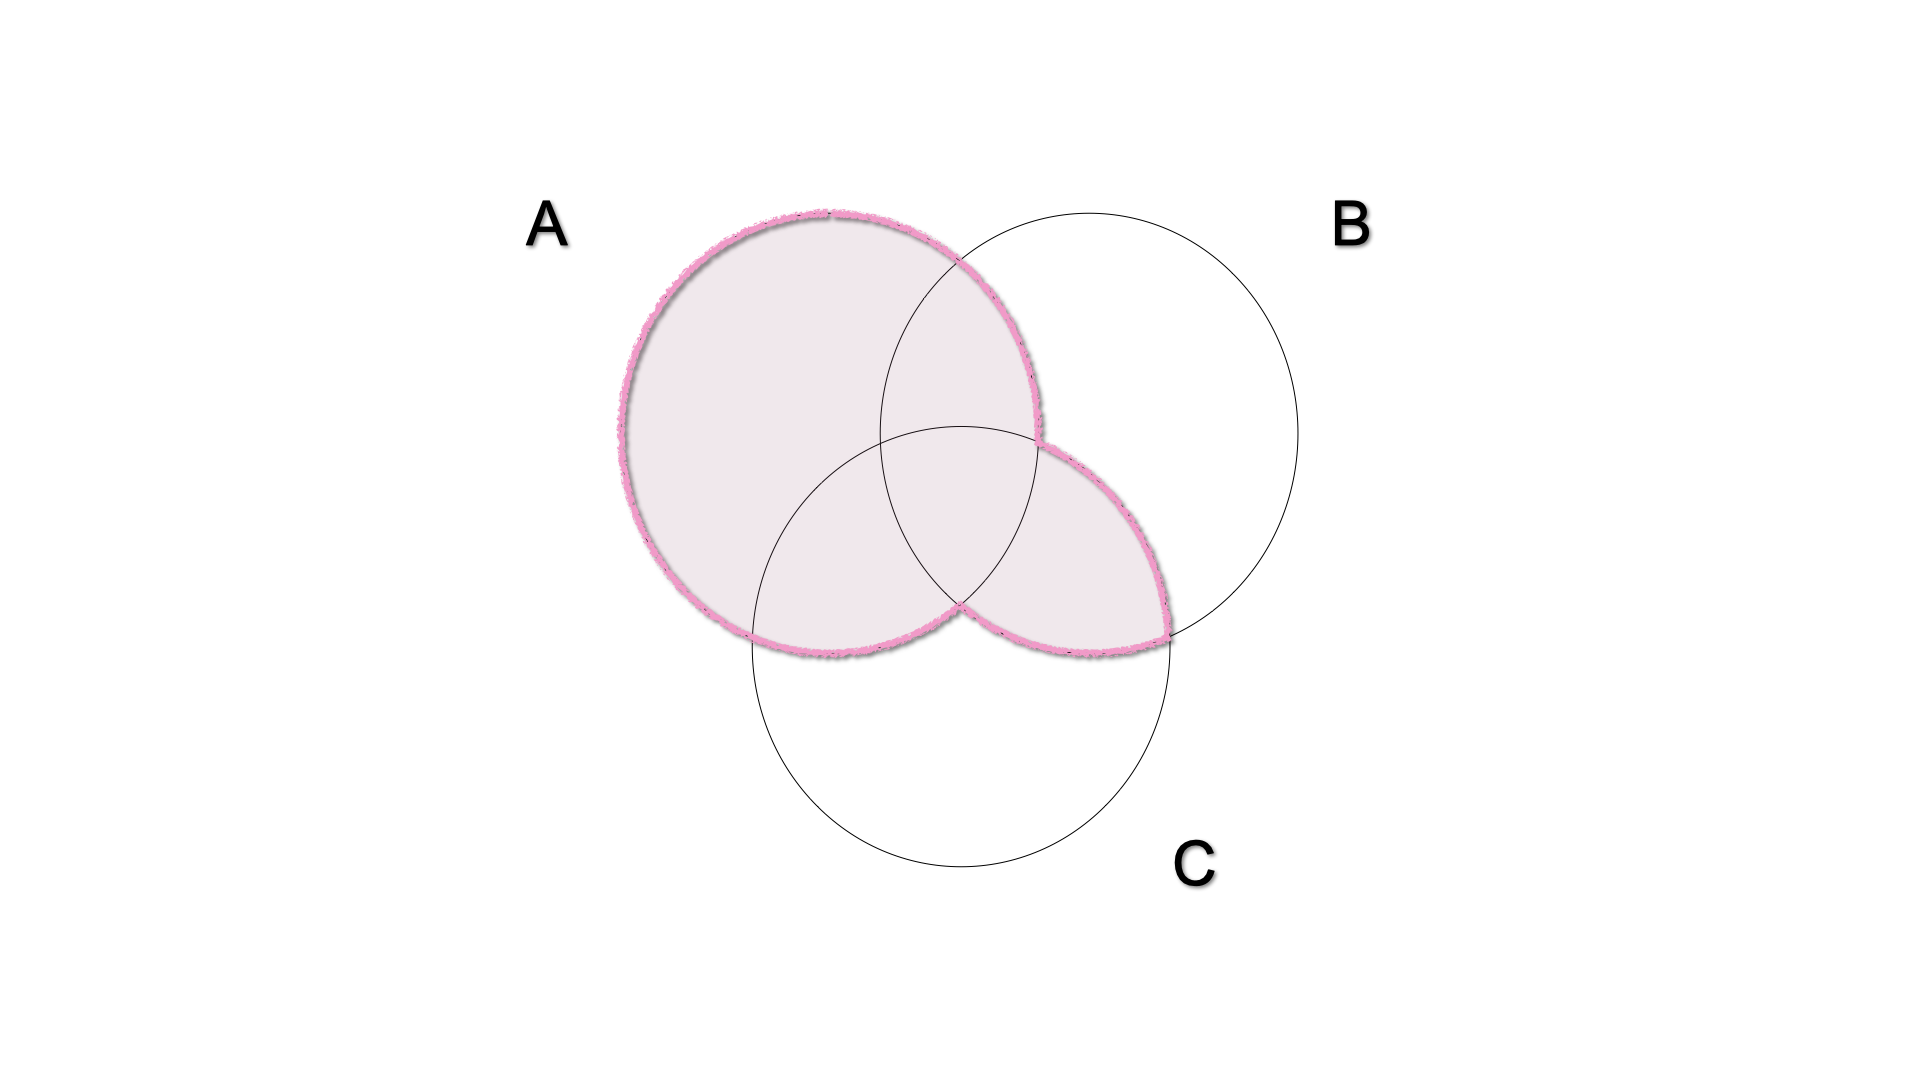
\includegraphics[scale=0.15]{img/charts/charts.009.png}
  \end{figure}
\end{frame}

% \begin{frame}
% \frametitle{Elements of set theory (Venn diagram)}
% ... for instance, let $A_1, A_2, A_3$ be in $S$ and let us introduce the shorthand notation:
% $$A_1 A_2 = A_1 \cap A_2  \quad \text{and} \quad A_1 A_3 = A_1 \cap A_3$$
% Then, we have:
% \begin{figure}[h!]
% \centering
% 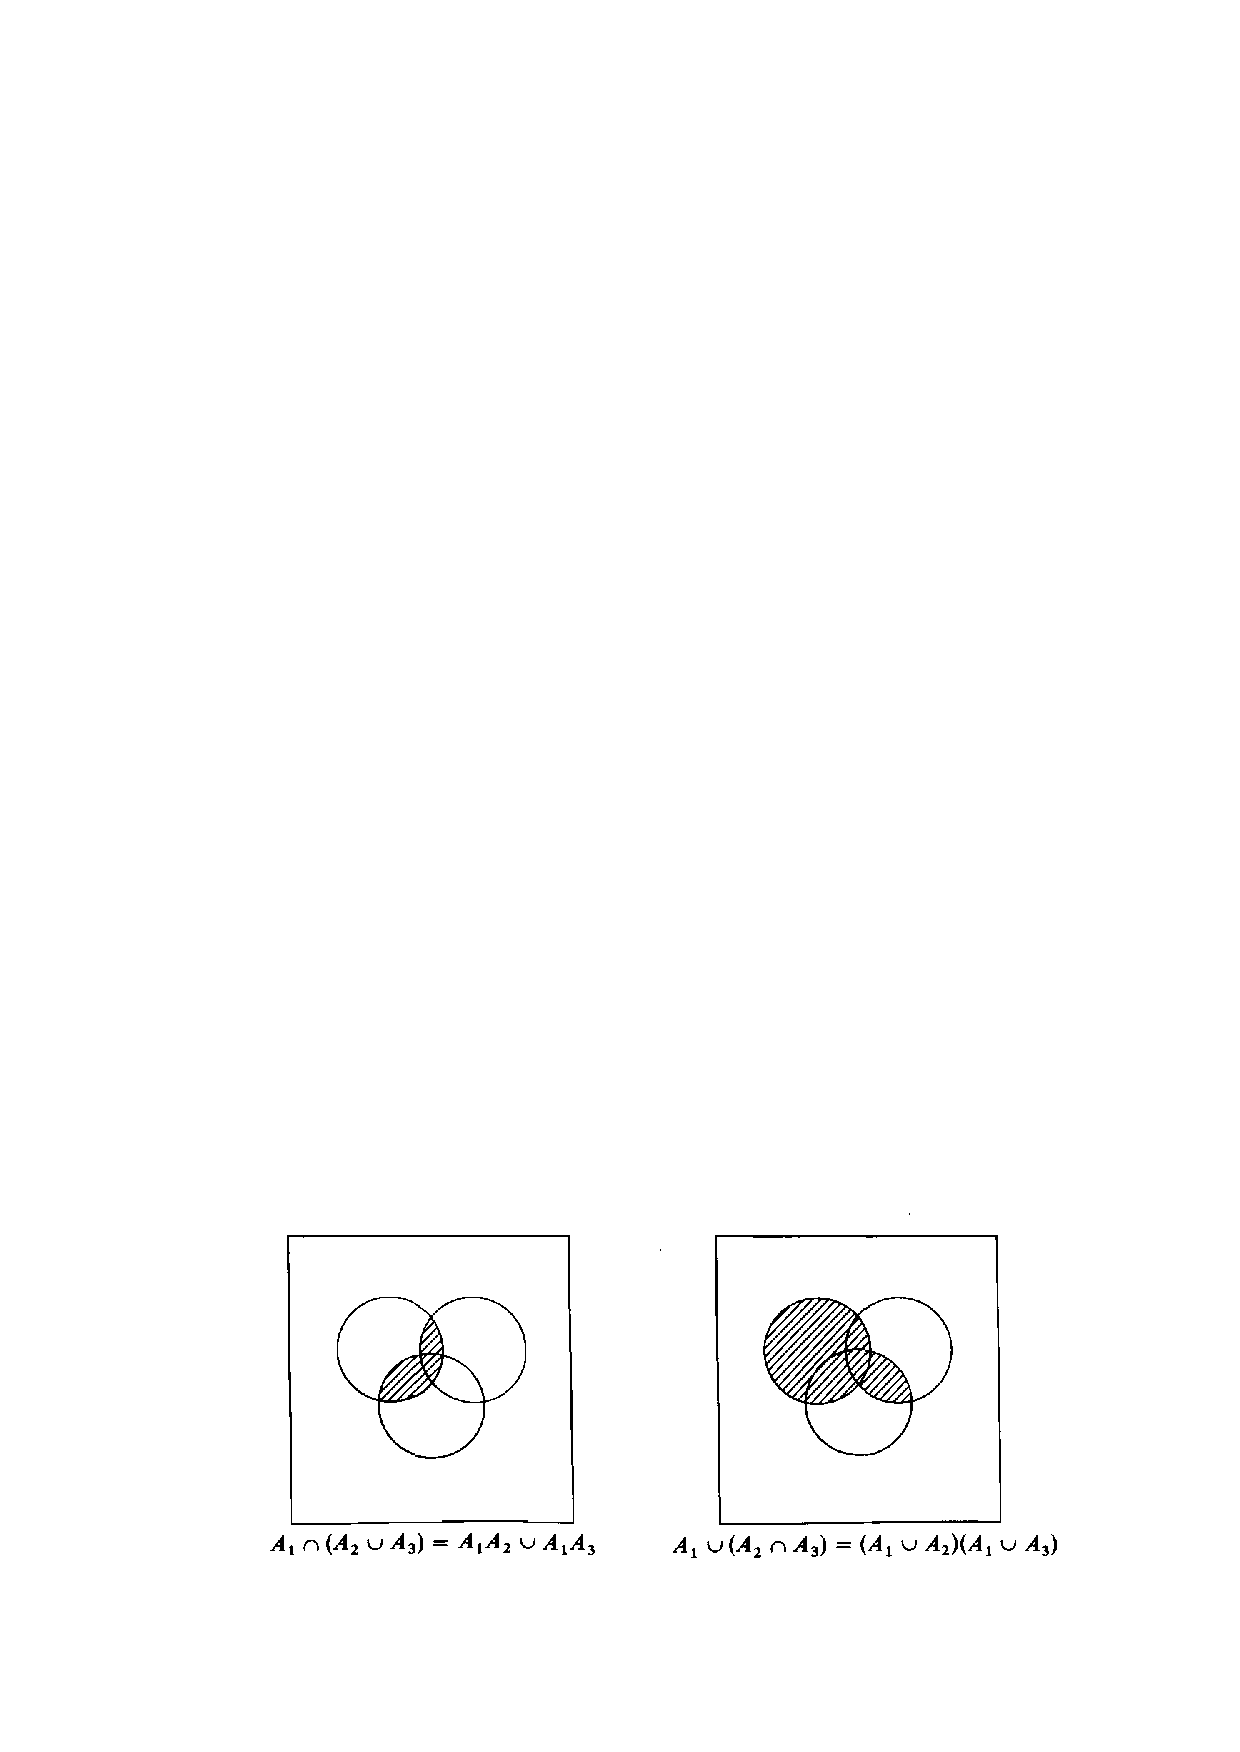
\includegraphics[width=0.9\textwidth,height=0.5\textheight]{img/commutative.pdf}
% \end{figure}
% \end{frame}


% \begin{frame}
% \frametitle{Elements of set theory (Venn diagram)}
% %\frametitle{Extra exercise (Venn diagram)}
% \begin{tiny}
% \begin{exercise}
% \def\firstcircle{(3,0) circle (1.5cm)}
% \def\secondcircle{(0:5cm) circle (1.5cm)}
%
% \colorlet{circle edge}{blue!50}
% \colorlet{circle area}{blue!20}
%
% \tikzset{filled/.style={fill=circle area, draw=circle edge, thick},
%     outline/.style={draw=circle edge, thick}}
%
% %Set A or B but not (A and B) also known a A xor B
% \hspace{1cm} (i)
% \begin{tikzpicture}\centering
%     \draw[filled, even odd rule] \firstcircle node {$A$}
%                                  \secondcircle node{$B$};
%     \node[anchor=south] at (current bounding box.north) {$\overline{A \cap B}$};
% \end{tikzpicture}
%
% \hspace{5cm} (ii)
% % Set B but not A
% \begin{tikzpicture}
%     \begin{scope}
%         \clip \secondcircle;
%         \draw[filled, even odd rule] \firstcircle
%                                      \secondcircle node {$B$};
%     \end{scope}
%     \draw[outline] \firstcircle node {$A$}
%                    \secondcircle;
%     \node[anchor=south] at (current bounding box.north) {$B - A$};
% \end{tikzpicture}
% \end{exercise}
% \end{tiny}
% \end{frame}

%%%%%%%%%%%%%%%%%%%%%%%%%%%%%%%%%%%%%%%%%%%%
\section{Countable and Uncountable Sets}
%%%%%%%%%%%%%%%%%%%%%%%%%%%%%%%%%%%%%%%%%%%%

\begin{frame}{\secname}

Sets can be either \textbf{countable} or \textbf{uncountable}.

\vspace{0.5cm}

\begin{itemize}
\item A \textcolor{blue}{countable set} is a set with the same number of elements as a subset of the set of natural numbers ($\mathbb{N}$).\\[0.5em]

\textit{It can be either \textbf{finite} or \textbf{countably infinite}}
  \begin{itemize}
  \item Its elements can be counted one a time i.e. using $1,2,3,..$
  \item The counting may never finish.
  \end{itemize}
\item We can't do the same with uncountable sets!
\end{itemize}
% G. Cantor introduced the term countable set, contrasting sets that are countable with those that are \color{blue} uncountable
% \color{black} (i.e., nonenumerable or nondenumerable).
\end{frame}


\begin{frame}{\secname}
  \begin{example} [Countable and Finite sets]
  \begin{figure}[h!]
  \centering
  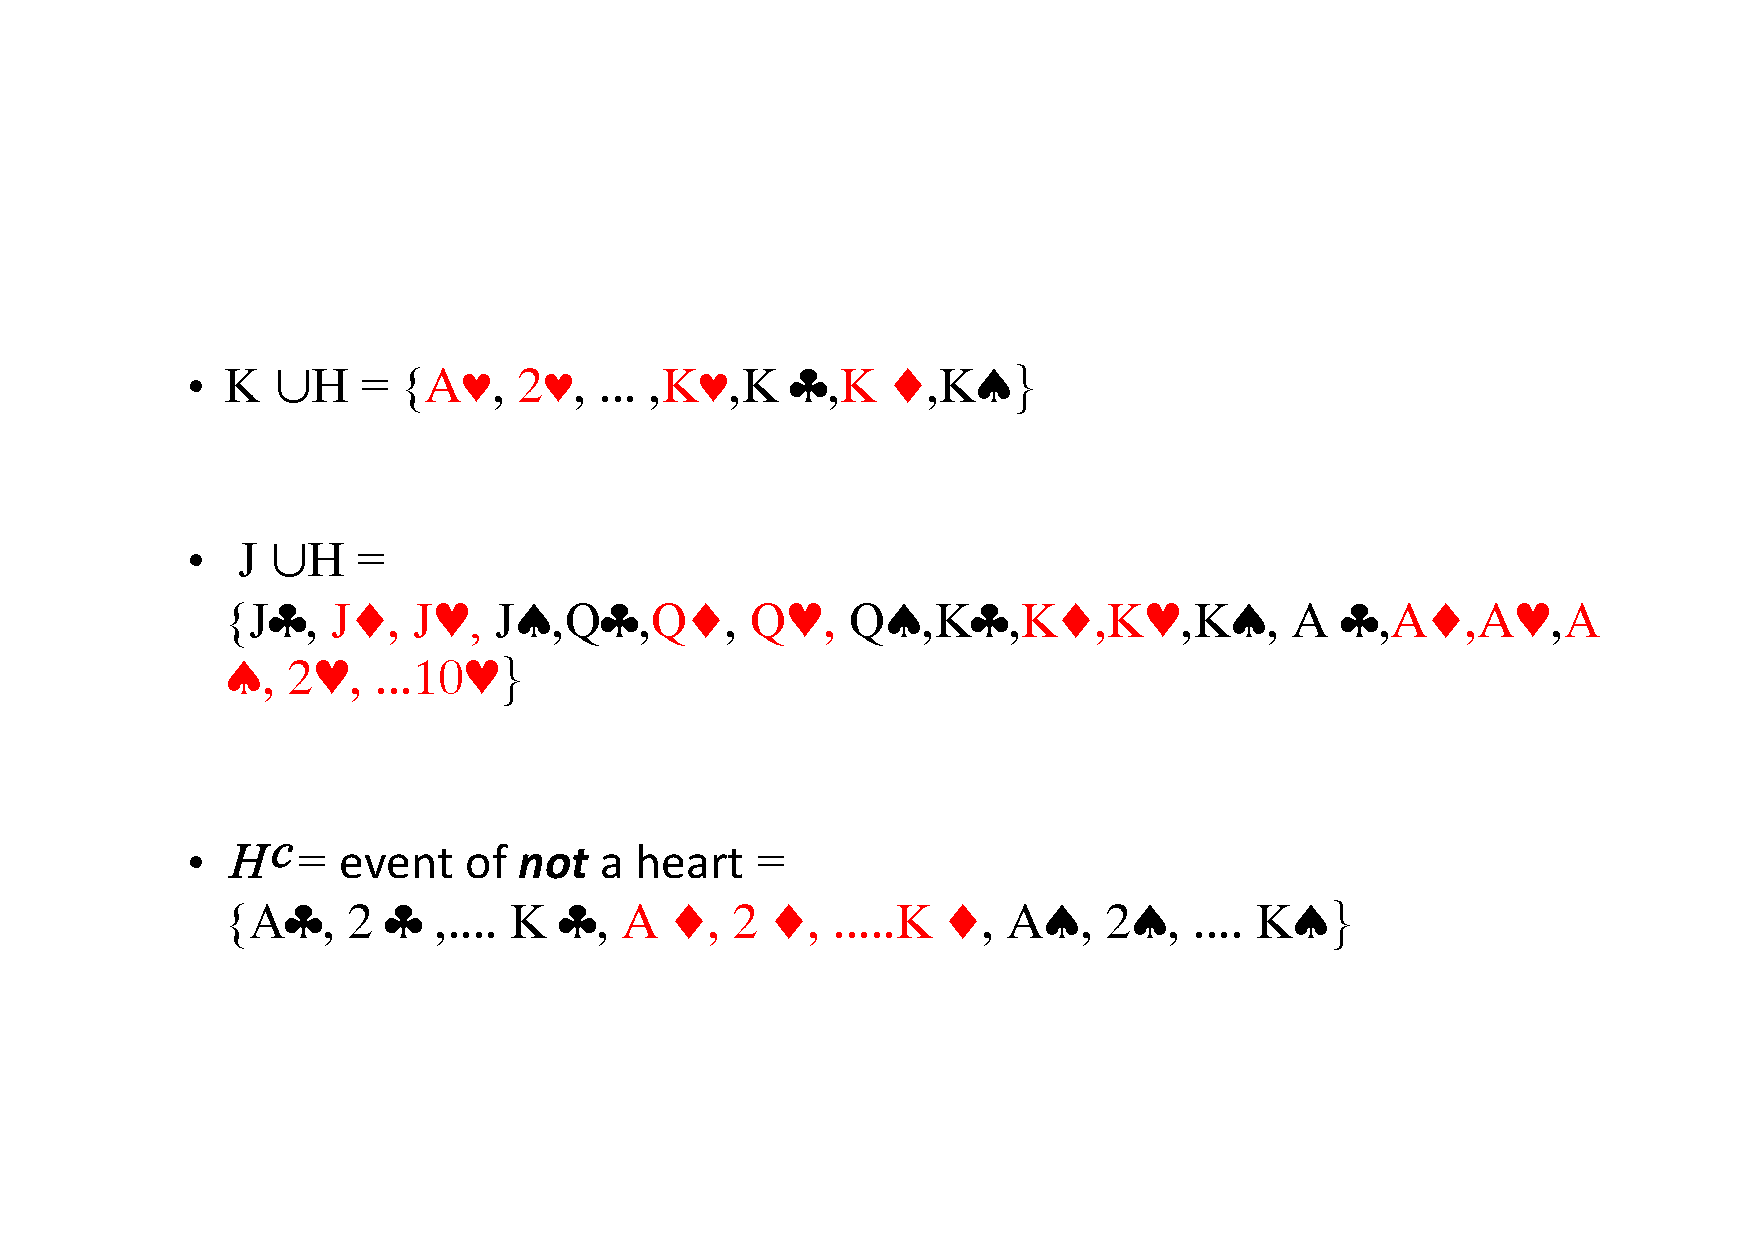
\includegraphics[scale=0.4]{img/Example2.pdf}
  \end{figure}
  \end{example}
\end{frame}

\begin{frame}{\secname}
  %Events can be represented by means of sets.
  \begin{exercise} [Uncountable]
  \begin{figure}[h!]
  \centering
  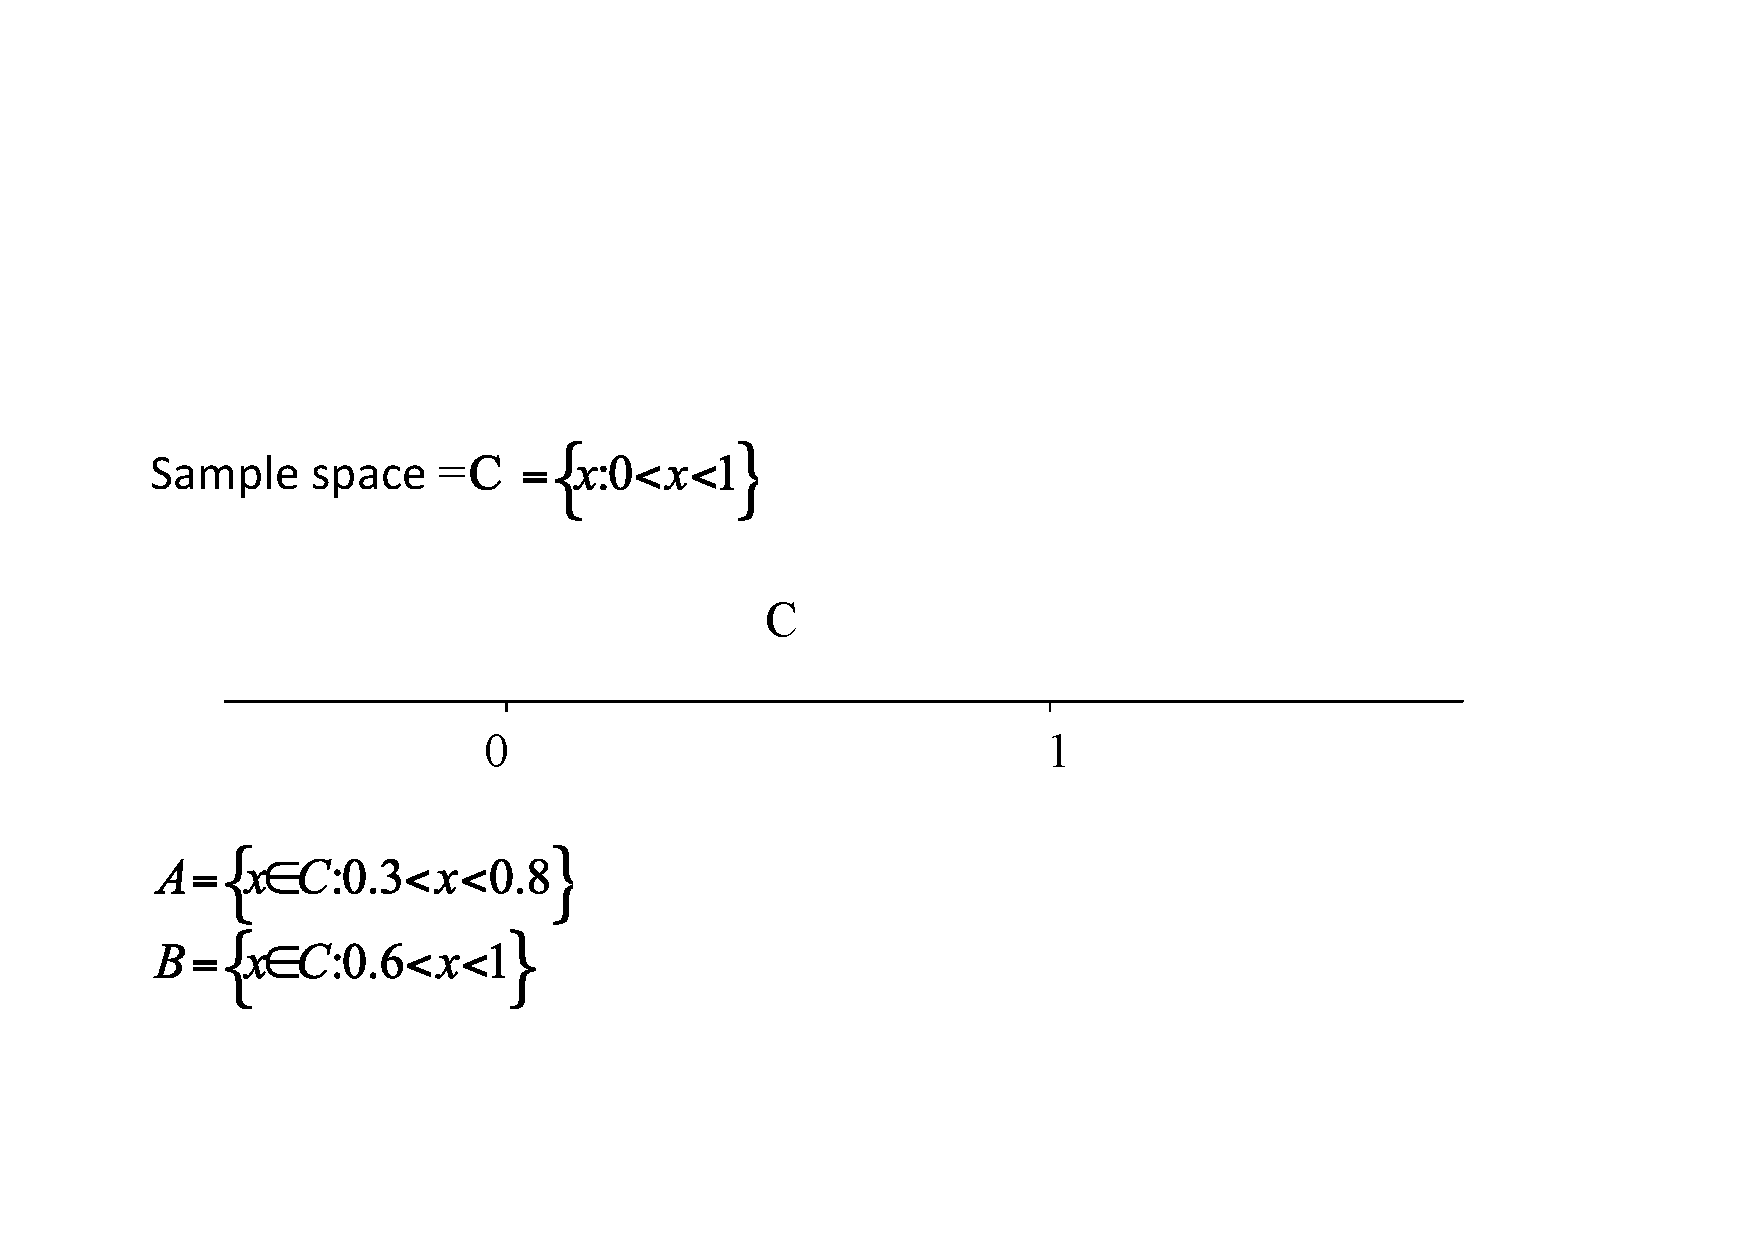
\includegraphics[width=0.9\textwidth,height=0.6\textheight]{img/Example3.pdf}
  \end{figure}
  \end{exercise}
\end{frame}


\begin{frame}{\secname}
  \begin{exercise}[cont'd]
  and using the definition of $A$ and $B$ compute:
  \begin{itemize}
  \begin{multicols}{2}
  \item $A^c$
  \item $B^c$
  \item $B^c \cup A$
  \item $B^c \cup A^c$
  \item $A \cup B$
  \item $A \cap B$
  \item $B \cup A^c$
  \item $A^c \cup A $
  \end{multicols}
\end{itemize}

%\begin{figure}[h!]
%\centering
%\includegraphics[width=0.6\textwidth,height=0.6\textheight]{Example3bis.pdf}
%\end{figure}
\end{exercise}
\end{frame}


\begin{frame}{\secname}
  \begin{exercise}[Countable]

  Let us consider the  experiment where we flip two coins. ($H$ stands for Head and $T$ for Tail).

  \vspace{0.5cm}
  $$ S = \Big\{ (HH),(HT),(TH),(TT)  \Big\}.$$ \\


  \vspace{0.5cm}

  Then, let us consider the events:
  \begin{itemize}
  \item $A= H$ is obtained at least once = $\Big\{ (HH),(HT),(TH) \Big\}$
  \item $B=$ the second toss yields $T$ =  $\Big\{ (HT),(TT) \Big\}$
  \end{itemize}
  %\begin{figure}[h!]
  %\centering
  %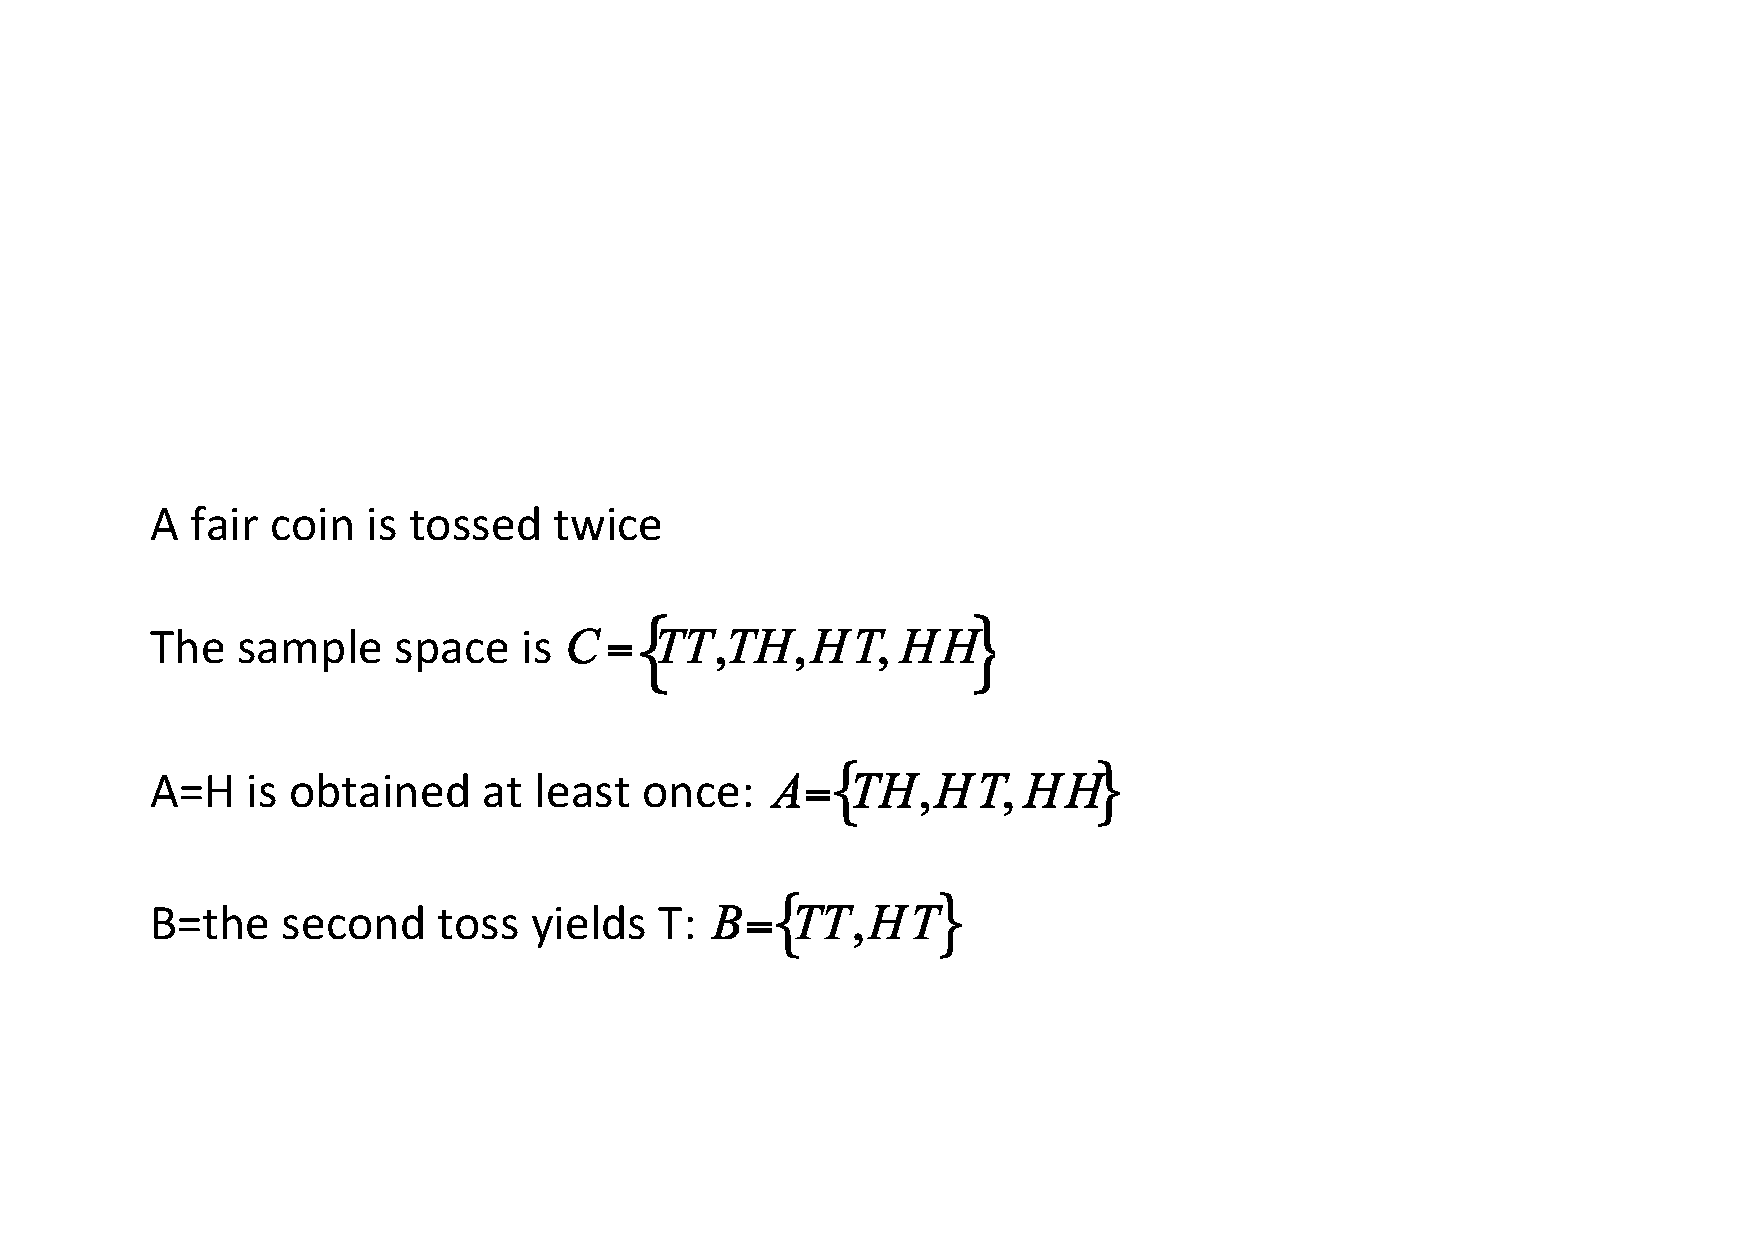
\includegraphics[width=0.9\textwidth,height=0.5\textheight]{Example4.pdf}
  %\end{figure}
  \end{exercise}
\end{frame}


\begin{frame}{\secname}
  \begin{exercise}[cont'd]
  and using the definitions of $A$ and $B$ compute:
  %\begin{figure}[h!]
  %\centering
  %\includegraphics[width=0.8\textwidth,height=0.5\textheight]{Example4bis.pdf}
  %\end{figure}
  \begin{itemize}
  \begin{multicols}{2}
  \item $A^c $
  \item $B^c$
  \item $B^c \cup A$

  \item $A \cup B$
  \item $A \cap B$
  \item $B \cup A^c$
  %\item $C^c$
  \end{multicols}
  \end{itemize}
  \end{exercise}
\end{frame}

\begin{frame}
  \frametitle{More on sets}
  \begin{exercise}[cont'd]
  and using the definitions of $A$ and $B$ compute:
  %\begin{figure}[h!]
  %\centering
  %\includegraphics[width=0.8\textwidth,height=0.5\textheight]{Example4bis.pdf}
  %\end{figure}
  \begin{itemize}
  \begin{multicols}{2}
  \item $A^c = \{ (TT) \}$
  \item $B^c = \{ (HH), (TH) \}$
  \item $B^c \cup A$

  \item $A \cup B$
  \item $A \cap B$
  \item $B \cup A^c$
  %\item $C^c$
  \end{multicols}
  \end{itemize}
  \end{exercise}
\end{frame}



\begin{frame}{\secname}
\begin{proposition}
Let $A\subset S$ and $\varnothing$ the empty set. The following relations hold:
\begin{itemize}
\begin{multicols}{2}
\item $A \cap S = A$;
\item $A \cup S = S$;
\item $A \cap \varnothing = \varnothing$;
\item $A \cup \varnothing = A$;
\item $A \cap A^c = \varnothing$;
\item $A \cup A^c = S$;
\item $A \cap A = A$;
\item $A \cup A = A$;
\end{multicols}
\end{itemize}
\end{proposition}
\pause
\begin{exercise}
Verify these relations using Venn diagrams.
\end{exercise}
\end{frame}

\begin{frame}{\secname}
  The above relations are helpful to define some other relations between sets/events.
  \begin{example}
  Let $A$ and $B$ be two sets in $S$. Then we have
  $$
  B = (B \cap A) \cup (B \cap A^c).
  $$
  To check it, we can proceed as follows:
  \bea
  B & = & S \cap B \nn \\
  \pause
   & = & (A \cup A^c) \cap B \nn \\
   \pause
   & = &  (B \cap A) \cup (B \cap A^c). \nn
  \eea
  \end{example}
\end{frame}

%%%%%%%%%%%%%%%%%%%%%%%%%%%%%%%%%%%%%%%%%%%
\section{De Morgan’s Laws}
%%%%%%%%%%%%%%%%%%%%%%%%%%%%%%%%%%%%%%%%%%%

\begin{frame}{\secname}
\framesubtitle{First Law}
  Let $A$ and $B$ be two sets in $S$. Then:
  \bea
  (A\cap B)^{c} =A^c \cup B^c,  \nn
  \eea

  where: \vspace{0.4cm}

  \begin{itemize}
\item Left hand side: \color{blue}$(A\cap B)^{c}$ \color{black} represents the \textbf{set of all elements that are not both $A$ and $B$}; \vspace
{0.4cm}
\item Right hand side:  \color{blue}$A^c \cup B^c$ \color{black} represents all elements that are not $A$ (namely they are $A^c$) and not $B$ either (namely they are $B^c$) $\Rightarrow$ \textbf{set of all elements that are not both $A$ and $B$}.
\end{itemize}
Put in words:
\begin{center}
The \textbf{complement of the Intersection} is the \textbf{Union of the Complements}
\end{center}
\end{frame}

\begin{frame}{\secname}
\framesubtitle{Second Law}

Let $A$ and $B$ be two sets in $S$. Then:
\bea
(A\cup B)^{c} =A^c \cap B^c,  \nn
\eea

where: \vspace{0.4cm}

\begin{itemize}
\item Left hand side: \color{blue}$(A\cup B)^{c}$ \color{black} represents the \textbf{set of all elements that are neither $A$ nor $B$}; \vspace
{0.4cm}
\item Right hand side:  \color{blue}$A^c \cap B^c$ \color{black} represents the intersection of all elements that are not $A$ (namely they are $A^c$) and not $B
$ either (namely they are $B^c$) $\Rightarrow$ \textbf{set of all elements that are neither $A$ nor $B$}.
\end{itemize}
\begin{center}
The \textbf{complement of the Union} is the \textbf{Intersection of the Complements}
\end{center}
\end{frame}


\begin{frame}{\secname}
\framesubtitle{Three sets}

These laws can be extended to \textbf{Three Sets}:\\[0.5em]

Let $A_{1}, A_{2}, A_{3} \subset S$, and  $A^{c}_{1} = \overline{A_{1}})$,\\[0.5em]

\begin{itemize}
\item[(i)] \textbf{First law}:
$$\overline{\left(A_{1}\cup A_{2}\cup A_{3}\right)} = \overline{A_{1}} \cap \overline{A_{2}} \cap \overline{A_{3}}$$
\item[(ii)] \textbf{Second Law}:
$$\overline{\left(A_{1}\cap A_{2}\cap A_{3}\right)} = \overline{A_{1}} \cup \overline{A_{2}} \cup \overline{A_{3}}$$
\end{itemize}

And to the union or intersection of \textbf{infinite sets} (see the Course notes)
\end{frame}

% \begin{theorem} [De Morgan]
% Let $\mathbb{N}$ be the set of natural number and $\{A_{i}\}$ a collection (indexed by $i \in \mathbb{N}$) of subsets of $S$. Then:
% \begin{itemize}
% \item[(i)]
% \bea
% \overline{\bigcup_{i \in \mathbb{N}} A_i} &=& \bigcap_{i \in \mathbb{N}} \overline{A}_i;
% \eea
% \item[(ii)]
% \bea
% \overline{\bigcap_{i \in \mathbb{N}} A_i} &=& \bigcup_{i \in \mathbb{N}} \overline{A}_i.
% \eea
%
% \end{itemize}
% \end{theorem}
% \end{frame}

%\begin{frame}
%\frametitle{Back to the events}
%
%
%The sample space of an experiment is denoted by $S$ and it is the complete listing of the elementary events (which are representable by means of
%sets) associated to a random experiment.
%\begin{example} [Countable]
%\begin{figure}[h!]
%\centering
%\includegraphics[width=0.8\textwidth,height=0.6\textheight]{Example11.pdf}
%\end{figure}
%\end{example}
%
%
%\end{frame}

%%%%%%%%%%%%%%%%%%%%%%%%%%%%%%%%%%%%%%%%%%%%%%%%%%%%%%%%
\section{Probability as Frequency}
%%%%%%%%%%%%%%%%%%%%%%%%%%%%%%%%%%%%%%%%%%%%%%%%%%%%%%%%

\begin{frame}{\secname}

\textbf{Primary interest} will be not in events  but on their \textcolor{blue}{\textit{likelihood}}.\\[0.5em]
\pause
Intuitively, the \textbf{"probability of an event"} is a \textbf{number associated to the event}:\\[0.5em]

$$\text{event} \rightarrow \text{pr(event)}$$

\pause
We would like this probability to feature the following properties:

\begin{enumerate}
\item To be \textbf{positive} or more generally non-negative (it can be zero);
\pause
\item The $\text{pr}(S)=1$ and $\text{pr}(\varnothing)=0$;
\pause
\item The probability of two (or more) \textbf{mutually exclusive events} is the \textbf{sum} of the probabilities of each event.
\end{enumerate}

\end{frame}

\begin{frame}{\secname}

In many experiments, it is natural to assume that all outcomes in the sample space ($S$) are equally likely to occur\\[0.5em]

For instance $S=\{1,2,3,...N\}$\\[0.5em]
\pause
\bea
P(\{1\})=P(\{2\})=...=P(\{N\}) \nonumber
\eea

or equivalently

$$P(\{i\})= \frac{1}{N}, \text{ for } i=1,2,...,N$$.

\pause

\begin{example}
\begin{center}
Think of when you throw a die!
\end{center}
\end{example}
\end{frame}


\begin{frame}{\secname}

If we define a \textbf{composite event $A$}, there exist $N_A$ realizations having the same likelihood (i.e. probability) in the event $A$, so:

$$\boxed{P(A)=\frac{N_A}{N}=\frac{\mbox{\# of favorable outcomes}}{\mbox{total \# of outcomes}}=\frac{\mbox{\# of outcomes in $A$}}{\mbox{ \# of outcomes in $S$}}}$$

(here $\# $ means ``number'').

\end{frame}


\begin{frame}{\secname}

\begin{example}
We roll a fair die and we define the event $$A=\text{the outcome is an even number}=\{2,4,6\}.$$
\textbf{What is the probability of $A$?}
\vspace{0.5cm}

\pause
Sample Space:
$$S=\{1,2,3,4,5,6\}.$$

%since the die is fair, each outcome is equally
%likely, so
%\bea
%\text{pr}(\{1\})=\text{pr}(\{2\})=...=\text{pr}(\{6\})=\frac{1}{6}. \nonumber
%\eea
%Thus, we conclude that
\pause
$$P(A)=\frac{N_A}{N} = \frac{\mbox{3 \text{favorable outcomes}}}{\mbox{6 total outcomes}} = \frac{1}{2}. %= \text{pr}(\{1\})+\text{pr}(\{2\})+\text{pr}(\{3\})
$$


\end{example}


\end{frame}


\begin{frame}{\secname}

Building on this intuition we state a first \textbf{informal definition of probability}, namely in terms of \textit{relative frequency}.

\pause

\begin{definition}[Informal]
An experiment with sample space is $S$, is repeatedly performed under exactly the same conditions.

For each event $A\subset S$, let $n(A)$ the \textbf{number of times $A$ occurs} in the \textbf{first $n$ repetitions} of the experiment.

\pause

Then, the \textbf{probability of the event $A$} is:
$$
P(A)=\lim_{n \to \infty} \frac{n(A)}{n},
$$
\end{definition}
% In words:
% $P(A)$ is the \textbf{limiting proportion}/frequency of times that $A$ occurs or the limit of the relative frequency of $A$.
\end{frame}

\begin{frame}{\secname}
\begin{example}[Tossing a well-balanced coin]

\begin{itemize}
\item 2 mutually exclusive equiprobrable outcomes: $H$ and $T$.
\item Let $A = \{H\}$, $P(A)=1/2$.
\item We can toss the coin a large number of times (each under identical conditions) and count the times we have H.
\end{itemize}

Let $n$ \textbf{total \# of tosses} and $n(A)$ the \textbf{\# of times in which we observe $A$}.
% Then, the relative frequency:
% $$\lim_{n \to \infty} \frac{n(A)}{n} \longrightarrow P(A) $$
Thus $$P(A) \sim \frac{n(A)}{n}, \quad \text{for large $n$}.$$
\end{example}
\end{frame}


\begin{frame}{\secname}
\begin{example}[cont'd]

\begin{figure}[h!]
\centering
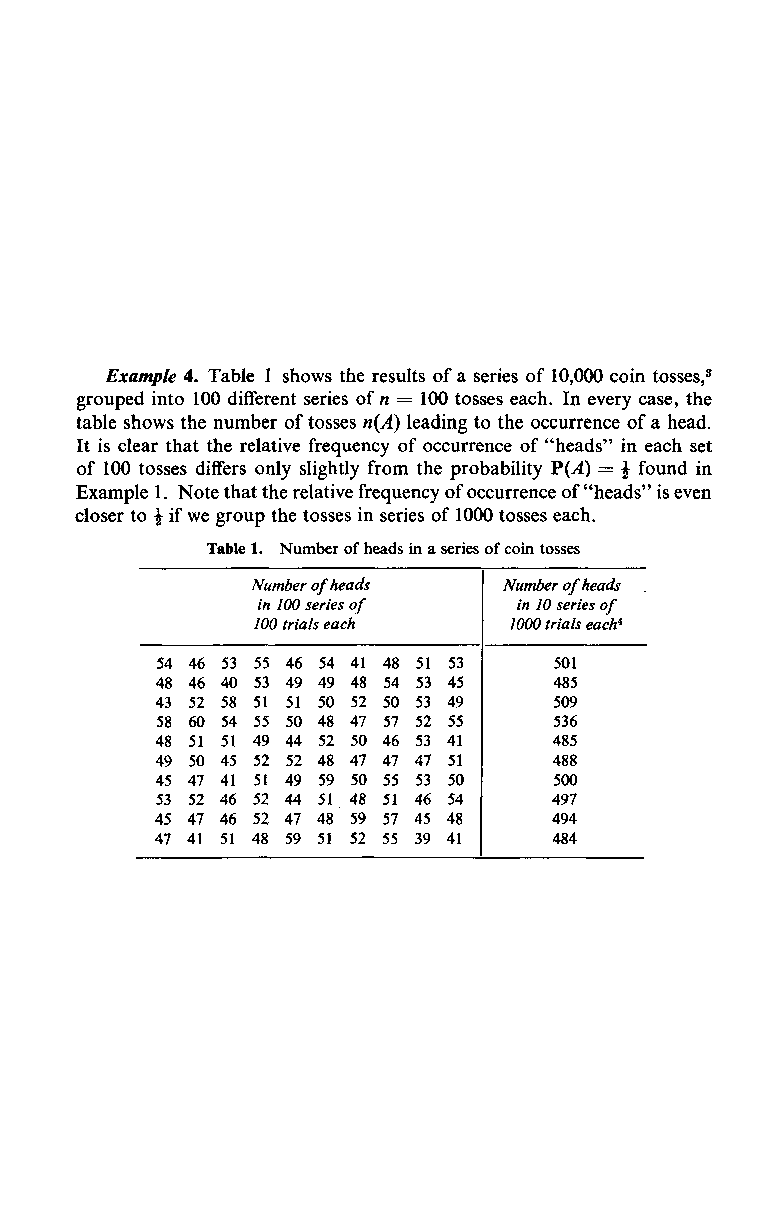
\includegraphics[width=0.7\textwidth,height=0.7\textheight]{img/roz.pdf}
\end{figure}
\end{example}
\end{frame}
%
%\begin{frame}
%\frametitle{Back to the events}
%
%Clearly,
%$$0 \leq n(A) \leq n, \quad \text{so} \quad  0 \leq P(A) \leq 1.$$
%Thus, we say that  \color{blue} the probability is a set function (it is defined on sets) and it associates to each set/event a number between zero and one.
%\color{black}
%
%\vspace{0.5cm}
%
%Now, let us recall that a real-valued function is a mapping from $D_f$ to $\mathbb{R}$ and we write:
%$$
%f \quad : \quad D_f \to \mathbb{R},
%$$
%where $D_f$ is the domain of $f$ and $\mathbb{R}$ is the range. \\
%
%\vspace{0.5cm}
%
%\color{red} \textbf{Q.} \color{black} In the case of the (function) probability, we already know that the range is $[0,1]$, but what about $D_f$?
%
%\end{frame}
%
%
%
%\begin{frame}
%\frametitle{Back to the events}
%
%To define $D_f$ for
%the probability, we have to rely on the set theory --- indeed $D_f$ has to be related to sets/events. To this end,
%%\vspace{0.3cm}
%\begin{definition} [$\sigma$-algebra]
%The $\sigma$-algebra $\mathcal{B}$ generated by the sample space $S$ is defined as the collection of all subsets of $S$ satisfying:
%\begin{enumerate}
%\item[(i)] $S \in \mathcal{B}$;
%\item[(ii)] if $A \in \mathcal{B}$, then $A^c \in \mathcal{B}$;
%\item[(iii)] if $A_1 \in \mathcal{B}$ and $A_2 \in \mathcal{B}$, then $A_1 \cup A_2 \in \mathcal{B}$. More generally, for a collection of events $\{A_i\}$, with $i \in \mathbb{N}$, we have
%\bea
%A = \bigcup_{i \in \mathbb{N}} A_i \text{ \ is such that \ }  A \in \mathcal{B}. \nn
%\eea
%
%\end{enumerate}
%\end{definition}
%
%Thus,  we will have that
%$$
%\boxed{P \quad : \quad \mathcal{B} \to [0,1]. }
%$$
%
%\end{frame}
%
%
%\begin{frame}
%\frametitle{Back to the events}
%
%%In this way, we define the domain of the probability. Then,
%To provide a formal definition of probability, we will make use of $\mathcal{B}$ and we will need to impose some additional conditions (that we are going to call \textit{axioms}). \\
%\vspace{0.5cm}
%We here briefly state the ideas, then we will formalize them: \\
%\vspace{0.3cm}
%(i) When we define the probability we would want the have a domain (namely $\mathcal{B}$) such that it includes the
%sample space $S$, and $P(S)=1$. \\ \vspace{0.1cm}
%(ii)  Moreover, for the sake of completeness, if $A$ is an event and we can talk about the probability that $A$ happens, then it is
%suitable for us that $A^c$ is also an event in $\mathcal{B}$, so that we can talk about the probability that $A$ does not happen. \\ \vspace{0.1cm}
%(iii) Similarly, if
%$A_1$ and $A_2$ are two events (so we can say something about their probability of happening), so we should be able to say something about the probability of the event $A_1 \cup A_2$.
%
%
%\end{frame}


\begin{frame}{\secname}

Clearly,
$$0 \leq n(A) \leq n, \quad \text{so} \quad  0 \leq P(A) \leq 1.$$

Thus, we say that:

\begin{center}
\textcolor{blue}{the probability is a \textbf{set function}\footnote{A function that operates on a Set} that \textbf{associates a number between 0 and 1} to each set/event.}
\end{center}

\pause

Next week:

We'll further formalise this notion, by adding \textbf{conditions} to the three desired properties\dots
\end{frame}


%%%%%%%%%%%%%%%%%%%%%%%%%%%%%%%%%%%%%%%%%%%%%%%%%%%%%
% Next week I should start with this
%%%%%%%%%%%%%%%%%%%%%%%%%%%%%%%%%%%%%%%%%%%%%%%%%%%%%

% \vspace{0.15cm}
% \begin{remark}
% One can provide a more rigorous definition of probability, as a real-valued function which defines a mapping between sets/events and the interval $[0,1]$. To achieve this goal one needs the concept of sigma-algebra (which represents the domain of the probability), but we do not pursue with that---at the cost of losing the mathematical rigour of the next slide!!
% \end{remark}

% \begin{frame}{Spoilers for next week }
%   To express the probability,  we need to impose some additional conditions, that we are going to call \textbf{\textit{axioms}}. \\
%   \vspace{0.5cm}
%   We here briefly state the ideas, then we will formalize them: \\
%   \vspace{0.3cm}
%   (i) When we define the probability we would want the have a domain such that it includes the
%   sample space $S$ and $P(S)=1$. \\ \vspace{0.1cm}
%   (ii)  Moreover, for the sake of completeness, if $A$ is an event and we can talk about the probability that $A$ happens, then it is
%   suitable for us that $A^c$ is also an event, so that we can talk about the probability that $A$ does not happen. \\ \vspace{0.1cm}
%   (iii) Similarly, if
%   $A_1$ and $A_2$ are two events (so we can say something about their probability of happening), so we should be able to say something about the probability of the event $A_1 \cup A_2$.
% \end{frame}

\begin{frame}
\frametitle{Wrap-up}

  \begin{itemize}
  \item \textbf{Random Experiments}, have uncertain outcomes that define \textbf{Events} belonging  belonging to a \textbf{Sample Space}.
  \item Events and Sample Space are characterised as \textbf{Sets}.
  \item \textbf{Set Theory}, its notations and properties \textbf{is useful to understand events}.
  \item \textbf{Probability} can be first seen as the \textbf{proportion of favorable occurrences} of equiprobable, mutually exclusive events over the number of \textbf{possible outcomes}.
  \item \textbf{Probability} can also be seen as the \textbf{limiting proportion} of occurrences of an event when \textbf{the experiment is repeated}.
  \end{itemize}
\end{frame}


\begin{frame}
	\begin{center}

		\LARGE{Thank you for your attention!}

		\pause

		\LARGE{``See you" next week!}
	\end{center}
\end{frame}

\end{document}

